%%%%%%%%%%%%%%%%%%%%%%%%%%%%%%%%%%%%%%%%%%%%%%%%%%%%%%%%%%%%%%%%%%%%%%%%%%%
% Trim Size : 11in x 8.5in
% Text Area : 9.6in (include Runningheads) x 7in
% ws-ijbc.tex, 24 Jan 2010
% Tex file to use with ws-ijbc.cls written in Latex2E.
% The content, structure, format and layout of this style file is the
% property of World Scientific Publishing Co. Pte. Ltd.
%%%%%%%%%%%%%%%%%%%%%%%%%%%%%%%%%%%%%%%%%%%%%%%%%%%%%%%%%%%%%%%%%%%%%%%%%%%
%

%\documentclass[•]{•}ass[draft]{ws-ijbc}
\documentclass{ws-ijbc}
\usepackage{ws-rotating}     % used only when sideways tables/figures are used
\usepackage{epstopdf}
\usepackage{mathrsfs}
\usepackage{graphicx}
\usepackage{float}
\usepackage{bm}
\bibliographystyle{ws-ijbc}
\newcommand{\norm}[1]{\left\lVert#1\right\rVert}

\makeatletter
\newcommand*{\getlength}[1]{\strip@pt\dimexpr0.035136\dimexpr#1\relax\relax}
\newcommand{\showfont}{%
encoding: \f@encoding{},\\
family: \f@family{},\\
series: \f@series{},\\
shape: \f@shape{},\\
size: \f@size{} pt,\\
text height: \getlength{\the\textheight} cm,\\
text width:     \getlength{\the\textwidth} cm}
\makeatother


\begin{document}

\catchline{}{}{}{}{} % Publisher's Area please ignore

\markboth{Elle Musoke, Bernd Krauskopf, and Hinke M. Osinga}{A Heteroclinic Connection between Two Saddle Slow Manifolds in the Olsen Model}

\title{A Heteroclinic Connection between \\ Two Saddle Slow Manifolds in the Olsen Model}

\author{Elle Musoke, Bernd Krauskopf, and Hinke M. Osinga}


\address{Department of Mathematics, University of Auckland, Private Bag 92019\\
Auckland, 1142, New Zealand\\
elle.musoke@auckland.ac.nz}

\maketitle

\begin{history}
\received{(to be inserted by publisher)}
\end{history}

\begin{abstract}
The abstract should summarize the context, content and conclusions
of the paper. It should not contain any references or displayed
equations. Typeset the abstract in 10~pt Times Roman with
baselineskip of 12 pt, making an indentation of 1.6~cm on the left
and right margins.
\end{abstract}

\keywords{A list of 3--5 keywords are to be supplied.}
\section{Introduction}

Multiple-time scale dynamical systems are characterized by certain variables evolving on a fast time scale while other variables evolve on a slower time scale.  The separation of variables into fast and slow can be found in many systems: chemical systems, neurons, electric circuits, lasers, and predator-prey dynamics, among others, have been described by slow-fast models  \cite{BZ_reaction, Neurons, Circuits, lasers, Predator-Prey}.  In \cite{BZ_reaction}, oscillations in the Belousov-Zhabotinsky reaction arise as a consequence of time-scale splitting.  Slow-fast models for neurons are studied in \cite{Neurons} in which different time scales result in neural excitability.  One of the most famous slow-fast systems is presented in \cite{Circuits} in which time-scale splitting again causes oscillations in a circuit.  Lasers can also be modelled with slow-fast systems as shown in \cite{lasers} which investigated interspike interval length.  A more ecological example can be found in \cite{Predator-Prey} which uses a slow-fast model to investigate the effect of a changing predator diet on predator-prey dynamics.  By reason of their ubiquity, various phenomena that arise from the multiple-time-scale nature of slow-fast systems are of significant interest. These have been described for two- and three-dimensional systems by well-established theory \cite{canard_explosion, lents-rapides, enlacement,singular_hopf, folded_node,three}.

We are concerned here with mechanisms responsible for the oscillatory behaviours exhibited by many slow-fast systems.  In two-dimensional systems canard explosions, small-amplitude limit cycles transitioning to larger-amplitude relaxation oscillations were studied, for example, in the Van der Pol oscillator and the FitzHugh--Nagumo model \cite{canard_explosion, fitz-hugh-nagumo}.  In three-dimensional systems, periodic orbits (POs) with epochs of localized small-amplitude oscillations (SAOs) and epochs of large-amplitude oscillations (LAOs) have been observed \cite{BZ}.  The mechanisms that cause SAOs of these appropriately named mixed-mode oscillations (MMOs) are described in \cite{MMO} for three-dimensional systems.  In this paper, we investigate novel phenomena that arise in four-dimensional slow-fast systems which may provide insight into undiscovered mechanisms for MMOs in higher-dimensional systems.

Previous studies exploring the mechanisms for MMOs in slow-fast dynamical systems investigate the role of so-called slow manifolds in the MMOs' generation and organisation \cite{Vo_paper, Vo_paper2, Emily_Harvey_paper, Martin_neuron_paper, Cris_paper}.  Slow manifolds are families of trajectories on which the flow evolves on the slow timescale.  A slow manifold may have families of trajectories that converge toward it in forward or backward time, respectively called the stable and unstable manifolds of the slow manifold.  Slow manifolds may have both a stable and an unstable manifold in which case we say it is a saddle slow manifold.  

Literature concerning slow manifolds explores slow manifolds and systems of, respectively, varying dimensions. Endocrine pituitary cells were studied with a four-dimensional slow-fast model that had a two-dimensional slow manifold in \cite{Vo_paper2}.  In \cite{Emily_Harvey_paper} a three-dimensional slow manifold was studied in a four-dimensional model for calcium oscillations inside cells. In \cite{Vo_paper} a four-dimensional model for a pituitary lactotropic cell was investigated from both a two- and three-timescale viewpoints.  From the two-timescale perspective, the model has a three-dimensional slow manifold.  In \cite{Martin_neuron_paper} a six-dimensional model for an excitable neuron was investigated.  The model had a two-dimensional slow manifold which plays a role in the generation of oscillations in the system.  A five-dimensional model with a one-dimensional slow manifold was also investigated.  In \cite{Saeed_Paper} techniques were developed to compute stable and unstable manifolds of one-dimensional saddle slow manifolds in three-dimensional systems. In \cite{Cris_paper}, these techniques were generalised to compute a two-dimensional saddle slow manifold and its two-dimensional stable and unstable manifolds in the four-dimensional Hodgkin--Huxley model.  To our knowledge, there is no literature on the computation of three-dimensional (un)stable manifolds of one-dimensional saddle slow manifolds at this time.

We consider a prototypical four-dimensional slow-fast dynamical system that exhibits MMOs, namely an Olsen model for peroxidase-oxidase reaction.  First introduced by Lars F. Olsen in 1983  \cite{Olsen}, there are currently many different versions of the Olsen model of different dimensions.  We consider the Olsen model in the form from \cite{Rescaling} and earlier work.  The MMO, denoted by $\Gamma$, in the Olsen model phase space is of particular interest because it does not seem to be generated by the mechanisms for MMOs familiar from three-dimensional systems.

The classification of variables into those that evolve on a fast time scale and those that evolve on a slow time scale is not straightforward for the Olsen model because the variables are not consistently slow or fast over all regions of phase space.  In fact, the Olsen model nominally has three different time scales.  We focus specifically on a parameter regime corresponding to two different time scales with three fast and one slow variables.  This parameter regime also corresponds to attracting $\Gamma$ and was the focus in \cite{QSSA}.  This study reported on mechanisms for $\Gamma$ after a model reduction to a three-dimensional system.  Two saddle slow manifolds were computed along with their stable and unstable manifolds.  These gave insight into the formation of the Olsen model MMO, as well as the cause of its particular geometry.  However, because of the assumptions used to reduce the model to a three-dimensional system, the dimensions of the stable manifold of one slow manifold and unstable manifold of the other were reduced to two in contrast to the corresponding three-dimensional manifolds in the full system.  

Examples of computing and visualising three-dimensional manifolds are in \cite{Initial_conditions_volume, Invariant_tori_again, Invariant_tori}.  None of these examples are in the context of computing (un)stable manifolds of saddle slow manifolds.  Tools to implement the computation of three-dimensional manifolds are not widely used at this time and, once computed, it is difficult to see the dynamics on the manifold in lower-dimensional projections.  Due to the nature of the current computation tools available, computing the entire three-dimensional manifold would also be computationally expensive compared to the the computation of two-dimensional manifolds.

In the full system, the three-dimensional stable manifold of one slow manifold and the three-dimensional unstable manifold of the other are expected to intersect generically in a two-dimensional surface of connections between the two slow manifolds.  Such a surface does not generically exist in four-dimensional systems for slow manifolds of dimension greater than one.  The surface of connections also does not exist generically in systems of dimension lower than four.  In these cases, the stable and unstable manifolds of the saddle slow manifolds are limited to dimensions of two or lower and therefore do not typically have robust intersections of dimension two or higher.  In this research, we generalise the techniques in \cite{Saeed_Paper} with the aim of computing the three-dimensional stable and unstable manifolds of the one-dimensional saddle slow manifolds in the Olsen model.  Furthermore, we use our techniques in conjunction with Lin's method to compute the intersection of the three-dimensional stable and unstable manifolds in the full four-dimensional model.  This intersection is involved in the formation and organisation of $\Gamma$ and could lead to insights about the formation and organisation of MMOs in other higher-dimensional systems.

This paper is organized as follows.  In the next section we give the necessary background from geometric singular perturbation theory (GPST) for defining the three-dimensional manifolds which are the focus of this research.  Section 3 gives definitions of the manifolds which are then computed.  In section 4, a computation of the intersection of the manifolds from section 3 is described for the case where the time-scaling parameter is greater than zero as well as for the case when the time-scaling parameter is equal to zero.  Section 5 gives an analysis of differences between the manifolds computed in section 4.  Conclusions are given in section 6.

%Background section
\section{The Olsen Model}

We consider the scaled system from \cite{Rescaling}, given as the system of ordinary differential equations
    
\begin{equation}
\begin{aligned}
\begin{cases}
\frac{dA}{dt} &= \mu - \alpha A - ABY, \\ \vspace{2mm}\\
\frac{dB}{dt} &= \varepsilon(1-BX - ABY), \\ \vspace{2mm}\\
\frac{dX}{dt} &= \lambda(BX - X^2 +3ABY - \zeta X + \delta), \\ \vspace{2mm}\\
\frac{dY}{dt} &= \kappa\lambda(X^2 - Y - ABY),
\end{cases}
\end{aligned}
\label{equation_1}
\end{equation}
    
\noindent
where $(A, B, X, Y)\in\mathbb{R}^{4}$ are positive concentrations of chemicals.  The system parameters are represented by the Greek letters appearing in (\ref{equation_1}) and these have the values given in Table 1.  With the minor modification, for notational convenience, of using $\varepsilon$ for $\varepsilon_{b}$ and $\frac{1}{\lambda}$ for $\varepsilon^{2}$, they are chosen to be as in \cite{Rescaling}.  The time-scaling parameters $\varepsilon$ and $\lambda$ are chosen so that we are dealing with a regime with three fast variables, $A$, $X$, and $Y$, and one slow variable, $B$.

\begin{table}[h]
\tbl{Parameters of system (\ref{equation_1}) as in \cite{Rescaling} so that $A$, $X$, and $Y$ are fast and $B$ is slow.}
{\begin{tabular}{c  c  c  c  c  c  c  c  c} \\[-2pt]
\toprule
$\alpha$ & $\delta$ & $\varepsilon$ & $\lambda$ & $\kappa$ & $\mu$ & $\zeta$ \\[6pt]
\hline\\[-2pt]
0.0912 & $1.2121 \times 10^{-4}$ & 0.0037 & 18.5281 & 3.7963 & 0.9697 & 0.9847\\[1pt]
\botrule
\end{tabular}}
\end{table}
    
The classical analysis of slow-fast systems considers the two singular limits, for example, \cite{MMO}.  In the limit of $\varepsilon = 0$, system (\ref{equation_1}) reduces to
    
\begin{equation}
\begin{aligned}
\begin{cases}
\frac{dA}{dt} &= \mu - \alpha A - ABY, \\ \\
\frac{dX}{dt} &= \lambda(BX - X^2 +3ABY - \zeta X + \delta), \\ \\
\frac{dY}{dt} &= \kappa \lambda(X^2 - Y - ABY),
\end{cases}
\end{aligned}
\label{equation_2}
\end{equation}
    
\noindent
with $\frac{dB}{dt}=0$, meaning that $B$ is a parameter of (\ref{equation_2}).  We refer to the three-dimensional system (\ref{equation_2}) as the fast subsystem.  Performing the time rescaling $\tau = \varepsilon t$ and then considering the limit of $\varepsilon = 0$, system (\ref{equation_1}) reduces to the differential algebraic reduced system
    
 \begin{equation}
\begin{aligned}
\begin{cases}
0 &= \mu - \alpha A - ABY, \\ \\
\frac{dB}{d\tau} &= (1-BX - ABY), \\ \\
0 &= \lambda (BX - X^2 +3ABY - \zeta X + \delta), \\ \\
0 &= \kappa \lambda(X^2 - Y - ABY).
\end{cases}
\end{aligned}
\label{equation_3}
\end{equation}
    
\noindent
The three algebraic equations in system (\ref{equation_3}) define a one-dimensional manifold, called the critical manifold, denoted $C$.

The critical manifold $C$ consists of equilibria of the fast subsystem (\ref{equation_2}), which exist in ($A$,$B$,$X$,$Y$)-space for different values of $B$.  Their stability can be determined from the eigenvalues of the $3\times3$ Jacobian matrix of (\ref{equation_2}) evaluated at each point on the critical manifold.  Points $p \in C$ at which the Jacobian of (\ref{equation_2}) has eigenvalues with non-zero real parts are called hyperbolic.  The eigenvectors associated with the eigenvalues are categorized based on the sign of the real part of the associated eigenvalue.  Eigenvectors whose associated eigenvalues have negative real parts are called stable directions of $p$ and these span the stable eigenspace $E^{s}(p)$ of $p$.  The unstable directions and the unstable eigenspace, $E^{u}(p)$, can be defined similarly by the eigenvectors associated with eigenvalues having positive real part.  Note that the dimensions of the stable and unstable eigenspaces are equal to the number of eigenvalues with negative and positive real parts respectively.  Equilibria at which the Jacobian has eigenvalues with zero real-part are called non-hyperbolic and these correspond to bifurcations of system (\ref{equation_2}) \cite{The_Kuz} .

\begin{figure}[!t]
\centering
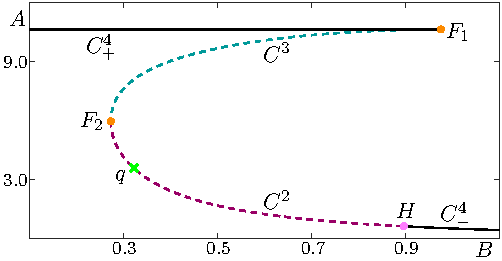
\includegraphics[]{./figures/MKMO_1.pdf}
\caption{Physically relevant branches $C^2$, $C^3$, $C^4_\pm$ of the critical manifold of (\ref{equation_1}) shown in projection onto the ($B$,$A$)-plane.  Branches $C^2$ (dashed, raspberry curve) and $C^3$ (dashed, teal curve) consist of saddles of (\ref{equation_2}) and $C^4_\pm$ (solid, black curve) consist of attractors of (\ref{equation_2}).  Superscripts indicate the dimension of the stable eigenspace of the branch and subscripts are used to distinguish between the two branches of attractors.  Branches are divided by saddle-node bifurcation points $F_1$ and $F_2$ (orange dots) and a Hopf point $H$ (pink dot).  Also shown is a saddle equilibrium $q$ (green cross) of (\ref{equation_1}) existing on $C^2$.  Parameters are as in Table 1.}
\label{figure_1}
\end{figure}

The critical manifold $C$ in ($A$,$B$,$X$,$Y$)-space is divided into branches by bifurcation points of the fast subsystem (\ref{equation_2}), so that points on each branch have the same dimensions of stable and unstable eigenspaces.  In other words, the branches of $C$ are one-parameter families in $B$ of hyperbolic equilibria of system (\ref{equation_2}).  We define the stable eigenspace $E^s(C^i)$ of a branch $C^i$ as the collection of stable eigenspaces of all the points on the branch.  The dimension of $E^s(C^i)$, hence, one plus than the dimension of the stable eigenspace of each point on the branch.  In our notation for branches, superscripts indicate the dimension in ($A$,$B$,$X$,$Y$)-space of the stable eigenspace of the branch.  Further, we use subscripts to distinguish the two branches on which equilibria have three-dimensional stable eigenspaces, that is, are attracting.  

Four branches of $C$ lie in the physically relevant region where all phase-space variables are positive, these are shown in Figure \ref{figure_1} in projection onto the ($B$,$A$)-plane.  The uppermost branch denoted $C^4_+$ (solid, black curve) consists of stable equilibria of (\ref{equation_2}).  It is separated from the branch of saddle equilibria denoted $C^3$ (dashed, teal curve), by a very sharp fold at the point $F_1$ (orange dot) at $B \approx 0.956$.  Folds of the critical manifold correspond to saddle-node bifurcations of system (\ref{equation_2}) with respect to the parameter $B$, these are points at which one of the real eigenvalues of the Jacobian evaluated at the point changes signs.  Another fold at $B \approx 0.273$ denoted $F_2$ (orange dot), separates $C^3$ from a lower branch of saddle equilibria denoted $C^2$ (dashed, raspberry curve).   The branch $C^2$ ends at a Hopf bifurcation $H$ (pink dot) at $B \approx 0.897$, where two complex-conjugate eigenvalues of the Jacobian pass through the imaginary axis of the complex plane.  To the right of $H$, there is again a stable branch of equilibria denoted $C^4_-$ (solid, black curve).

The point $q$ (green cross) on $C^2$ at $B \approx 0.323$ is an equilibrium of system (\ref{equation_3}) and is, hence, an equilibrium for the full system (\ref{equation_1}).  The equilibrium $q$ has a two-dimensional stable and two-dimensional unstable manifold, denoted $W^s(q)$ and $W^u(q)$, respectively.  The manifolds $W^{s}(q)$ and $W^{u}(q)$ consist of trajectories in ($A$, $B$, $X$, $Y$)-space that converge to $q$ in forward and backward time respectively.  To the right of $W^u(q)$, in the ($B$, $A$)-projection, the flow is from right to left near $C^2$.  To the left of $W^u(q)$, in the ($B$, $A$)-projection, the flow is from left to right near $C^2$.  The manifolds $W^{s}(q)$ and $W^{u}(q)$ can be computed with the methods in \cite{Red_book}; They are not depicted in Figure \ref{figure_1}, but are shown in Figure \ref{figure_10}.

Our interest is in the branches $C^3$ and $C^2$ because they are saddle objects of different type and are crucial for organising the phase space.  These branches of the critical manifold are invariant for $\varepsilon = 0$, but not for $\varepsilon > 0$.  However, they do persist as locally invariant manifolds called slow manifolds \cite{Fenichel}.  The associated slow manifolds are traditionally denoted $S^3_\varepsilon$ and $S^2_\varepsilon$ but, for notational convenience, we drop the subscript indicating dependence on $\varepsilon$ and refer to these slow manifolds for $\varepsilon > 0$ simply as $S^3$ and $S^2$.  The slow manifold $S^3$ has the same dimension and stability and lies at an $O(\varepsilon)$ Hausdorff distance from $C^3$.  In particular, $S^3$ converges to $C^3$ as $\varepsilon \rightarrow 0$.  (For a definition of Hausdorff distance see, e.g., \cite{Hausdorff_Distance}.)  Orbit segments that lie on a slow manifold remain slow for $O(1)$ time with respect to the slow time scale.  It follows that any trajectory that remains slow for an $O(1)$ amount of slow time can be considered (to be on) a slow manifold.  However, eventually trajectories on a slow manifold may become fast. Due to their finite time nature, slow manifolds are not unique; however, any two slow manifolds lie exponentially close to each other in a suitable $O(\varepsilon)$ neighbourhood of $C$ \cite{Fenichel}.  To select unique representatives $S^3$ and $S^2$, we consider the slow manifold that remains slow for the longest amount of time in a specific numerical setup in section 3.

The Stable Manifold Theorem tells us that each $p \in C^3$ has a stable and an unstable manifold that are tangent to and have the same dimensions as $E^{s}(p)$ and $E^{u}(p)$, respectively.  We denote the stable manifold of a point $p \in C^3$ by $W^{s}(p)$ and its unstable manifold by $W^{u}(p)$.  We can then define the collection of stable manifolds for $p \in C^3$ as $W^{s}(C^3) = \bigcup_{p \in C^3} W^{s}(p)$, which is a three-dimensional manifold tangent to $E^s(C^3)$.  We can similarly define the three-dimensional unstable manifold $W^{u}(C^2)$ of $C^2$ which is tangent to $E^u(C^2)$.

According to Fenichel Theory, for $\varepsilon > 0$, the manifold $W^{s}(C^3)$ also persists in an $O(\varepsilon)$ neighbourhood as a three-dimensional local stable manifold $W^{s}_{loc}(S^3)$ of $S^3$.  The local stable manifold $W^{s}_{loc}(S^3)$ consists of families of trajectories that have a fast approach to $S^3$ then remain close to $S^3$ for $O(1)$ slow time.  The global stable manifold $W^{s}(S^3)$ can be obtained by extending $W^{s}_{loc}(S^3)$ backwards in time.  The three-dimensional unstable manifold $W^{u}(S^2)$ associated with $S^2$ is similarly defined for backwards time.  Again, due to the finite-time nature of the definitions for the three-dimensional manifolds $W^{s}(S^3)$ and $W^{u}(S^2)$, they are not unique.  To select unique representatives, we consider two-parameter families of orbit segments that remain slow for the longest amount of time subject to boundary conditions described in further sections.  
 
 %Saddle slow manifold section   
 \section{Computation of saddle slow manifolds and their (un)stable manifolds}

In \cite{Saeed_Paper} algorithms are presented for the computation of a one-dimensional saddle slow manifold and its (un)stable manifolds in a three-dimensional system.  We build on their work to define and compute unique representatives $S^3$ and $S^2$ as well as their stable and unstable manifolds, respectively.

\subsection{Definition of $S^3$}    
We define the slow manifold $S^3$ with respect to a closed interval $[B_{\mathrm{in}},B_{\mathrm{out}}]$ for the slow variable $B$.  The values for $B_{\mathrm{in}}$ and $B_{\mathrm{out}}$ are chosen such that $[B_{\mathrm{in}},B_{\mathrm{out}}] \subset (B_{F_1}, B_{F_2})$, where $B_{F_1}$ and $B_{F_2}$ are the $B$-values of the fold points $F_1$ and $F_2$, respectively.  Hence, for each $B_p \in [B_{\mathrm{in}},B_{\mathrm{out}}]$ there is a unique point $p=(p_A,p_B,p_X,p_Y) \in C^3$ such that $p_B = B_p$.  In the three-dimensional subsection $\{ \omega \in \mathbb{R}^4 \; | \; \omega_B=B_p\}$ we define a solid three-sphere $D^s_\delta(B_p)$ with radius $\delta$ and centre $p$ , given formally by

\begin{equation*}
D^s_\delta(B_p)=\{w \in \mathbb{R}^4 \; | \; w_B = B_p, \left\lVert w-p \right\rVert \leq \delta\}.
\end{equation*}    
\noindent
The union 
\begin{equation*}
\mathscr{D}^s = \bigcup\limits_{B_p \in [B_{\mathrm{in}}, B_{\mathrm{out}}]}^{} D^s_\delta(B_p)
\end{equation*}


\noindent
forms a four-dimensional compact cylinder.  The superscript $s$ indicates that   The radius $\delta$ is small, but it needs to be of $O(\varepsilon)$ to ensure that $S^3$ lies in $\mathscr{D}^s$.  The one-parameter family of orbit segments that enter $\mathscr{D}^s$ via $D_\delta(B_{\mathrm{in}})$ are candidates for $S^3$.   To select a unique representative $S^3$ we require that the orbit segment representing $S^3$ has maximal integration time in $\mathscr{D}^s$ while satisfying appropriate boundary conditions.  Our choice of boundary conditions is explained in section 3.2.
    
Figure \ref{figure_2} illustrates this definition with an enlargement of Figure \ref{figure_1} near the branch $C^3$, where we now sketch the relevant elements of this definition. The unique representative $S^3$, in projection onto the $(B,A)$-plane, enters $\mathscr{D}^s$ at $D^s_\delta(B_{\mathrm{in}})$ and exits at $D^s_\delta(B_{\mathrm{out}})$.

\begin{figure}[!t]
\begin{center}
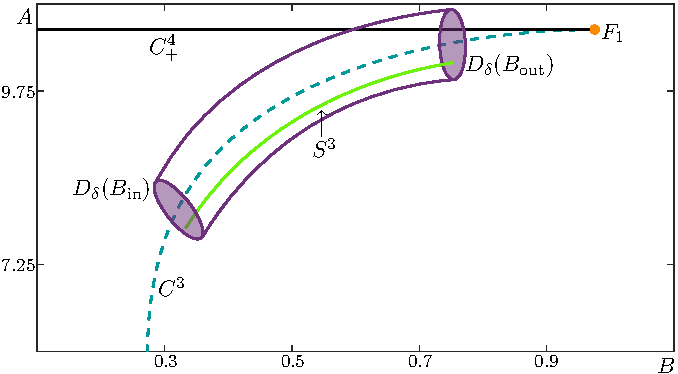
\includegraphics{./figures/MKMO_2.pdf}
\end{center}
\caption{A sketch of the unique representative slow manifold $S^3$ (green curve) projected into the ($B$,$A$)-plane.  The representative slow manifold $S^3$ is defined by having the longest integration time while entering and exiting  $D_\delta(B_{\mathrm{in}})$ and $D_\delta(B_{\mathrm{out}})$ (purple disks) at either end of a four-dimensional cylinder.  Also shown are $C^3$, $C^4_+$, and $F_1$.}
\label{figure_2}
\end{figure}

\subsection{Computation of $W^{s}(S^3)$ and  $S^3$}

Since $W^{s}(S^3)$ is three dimensional it is challenging to compute and difficult to visualise.  In fact, $W^{s}(S^3)$ can be represented as a two-parameter family of orbit segments that enter $\mathscr{D}^s$ at $D^s_{\delta}(B_p)$ for some $B_p \in [B_{\text{in}}, B_{\text{out}}]$, and remain inside $\mathscr{D}^s$ for $O(1)$ slow time.  A natural way forward is to consider $W^{s}(S^3)$ as a one-parameter family of two-dimensional submanifolds.  These submanifolds can be computed by generalizing the approach in \cite{Saeed_Paper}, which can then be implemented in the two-point boundary value problem (2PBVP) continuation package \textsc{Auto} \cite{AUTO}.  

Similarly to $S^3$, we select and approximate a specific candidate for $W^{s}(S^3)$ by requiring that each orbit segment lying on $W^{s}(S^3)$ has maximal integration time inside $\mathscr{D}^s$ and satisfies appropriate boundary conditions.  We now turn to the computation of the three-dimensional manifold $W^{s}(S^3)$ in the region where a corresponding two-dimensional stable manifold was investigated in the reduced model in \cite{QSSA}.

To select a submanifold we first define a two-dimensional plane $\Sigma$ that is transverse to the flow and to $E^u(C^3)$.  We can define $\Sigma$ by fixing $A$ and either $X$ or $Y$.  A smooth, one-parameter family of orbit segments of (\ref{equation_1}) is then given by the property that they begin in $\Sigma$, enter $\mathscr{D}^s$ at $D^s_{\delta}(B_p)$ for some $B_p \in [B_{\text{in}}, B_{\text{out}}]$, and remain inside $\mathscr{D}^s$ for $O(1)$ slow time.  We denote by $W^{s}_{\Sigma}$ the collection of those parts of these orbit segments that enter $\mathscr{D}^s$ in the fast direction.  The later parts that evolve mostly in the $B$-direction inside $\mathscr{D}^s$ for $O(1)$ slow time are approximate segments of $S^3$.  If such a later part of the orbit segment includes a fast exit from $\mathscr{D}^s$, the fast part lies on the unstable manifold $W^{u}(S^3)$ of $S^3$ in good approximation.

\begin{figure}[h]
\centering
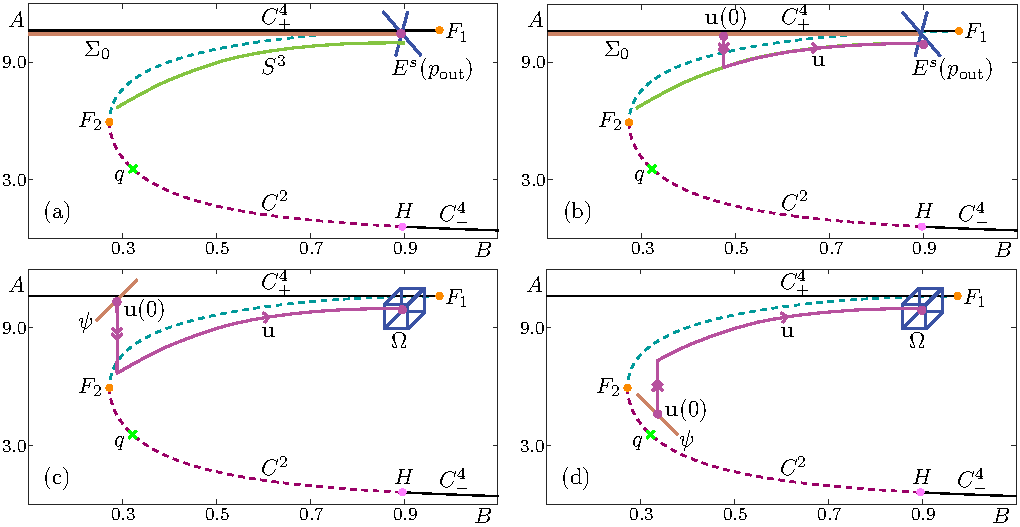
\includegraphics[]{./figures/MKMO_3.pdf}
\caption{A sketch in projection onto the ($B$,$A$)-plane of the numerical set-up for the computation of submanifolds of $W^s(S^3)$.  Also shown are $C^2$, $C^3$, $C^4_\pm$, $F_1$, $F_2$, $H$ and $q$.  Panel (a) shows a sketch at the start of the first homotopy step for computing $W^{s}_{\Sigma_0}$ with $S^3$ (a green curve), $E^s(p_{\text{out}})$ (blue cross), and the plane $\Sigma_0$ (mocha line) defined by the $A$- and $Y$-coordinates of the point $p_{\text{out}}$.  Panel (b) shows a representative orbit segment $\mathbf{u}$ (magenta curve) of the first homotopy step.  Panel (c) shows an illustration of the selection of a $\mathbf{u}$ with maximal integration time that starts at $\psi$ (mocha line) and ends on $\Omega$ (blue cube); here the one-dimensional subset $\psi \subset \Sigma_0$ is defined by fixing $B = B_{\text{in}}$ and $\Omega$ is spanned by $E^s(p_{\text{out}})$ and a vector in the $B$-direction. Panel (d) is a sketch of the selection of a different submanifold $W^{s}_{\Sigma}$ for $\Sigma$ on the other side of the critical manifold.}
\label{figure_3}
\end{figure}


We compute the submanifold $W^s_{\Sigma}$ as a one-parameter family of orbit segments $\mathbf{u} = \{\mathbf{u}(s) \;|\; 0 \leq s \leq 1 \}$ of the rescaled system

\begin{equation}
\frac{d\mathbf{u}}{ds} = TF(\mathbf{u}),
\label{equation_4}
\end{equation}
    
\noindent
where $\mathbf{u}(s) = (A(s), B(s), X(s), Y(s)) \in \mathbb{R}^4$ is the vector of chemical concentrations, $F$ is the right-hand side of (\ref{equation_1}) and $T$ is the total integration time on the fast timescale.  Orbit segments $\mathbf{u} \in W^s_{\Sigma}$ must satisfy the boundary conditions

 \begin{equation}
	\mathbf{u}(0) \in \Sigma,
	\label{general_conditions_1}
\end{equation}

\begin{equation}
	\mathbf{u}(1) \in \Omega = E^s(p_{out}) \times \begin{bmatrix} 0 & 1 & 0 & 0 \end{bmatrix}^{tr},
	\label{general_conditions_2}
\end{equation}

and

\begin{equation}
	T=T^{B}
	\label{general_conditions_3}
\end{equation}
where, for each $B_p \in \begin{bmatrix} B_{\text{in}} & B_{\text{out}} \end{bmatrix}$, $T^{B}$ is the maximum integration time of an orbit segment with $\mathbf{u}(0)_B=B_p$ satisfying (\ref{general_conditions_1}) and (\ref{general_conditions_2}).  Equations (\ref{general_conditions_1}), (\ref{general_conditions_2})  and (\ref{general_conditions_3}) define four conditions on solutions of (\ref{equation_4}) so that there is a one-parameter family of solutions to this 2PBVP.  Once an initial $\mathbf{u}$ satisfying (\ref{equation_4}), (\ref{general_conditions_1}), (\ref{general_conditions_2}), and (\ref{general_conditions_3}) is found, it is possible to sweep out the rest of $W^s_{\Sigma}$ by continuing $\mathbf{u}$ with varying $\mathbf{u}(0)_B$ and $T$.  The challenge in this type of set-up is generally the computation of an initial orbit segment that satisfies the boundary conditions.  For this purpose, we use homotopy steps as in  \cite{homotopy_example, Saeed_Paper}.

In the first homotopy step, we choose the point $p_{\text{out}}=\begin{pmatrix} p_A, p_B, p_X, p_Y \end{pmatrix}  \in C^3$ by fixing $p_B$ and the section $\Sigma=\Sigma_0=\{\omega \in \mathbb{R} \; | \;  \omega_A=p_A, \omega_Y=p_Y\}$, and define the boundary condition
\begin{equation}
	\mathbf{u}(1) \in E^s(p_{out}).
	\label{specific_BC}
\end{equation}
Then $\mathbf{u}(t)=p_{\text{out}}$ is a solution to (\ref{equation_4}), (\ref{general_conditions_1}), and (\ref{specific_BC}) with $T=0$.  In the second homotopy step, we continue the orbit segment $\mathbf{u}$ by increasing $T$ until $\mathbf{u}(0)_B$ is sufficiently small.  We then can perform a third homotopy step to move $\Sigma$ to a desired location.  In a final homotopy step, we impose the condition

\begin{equation}
	\mathbf{u}(0) \in \psi=\Sigma_{0} \cap \{ \omega \in \mathbb{R}^4 \; | \; \omega_B = B_{\text{in}} \}.
	\label{BCSTOP}
\end{equation}
By construction the $\mathbf{u}$ at the end of the previous homotopy step is a solution to (\ref{equation_4}), (\ref{general_conditions_2}), and (\ref{BCSTOP}).  Integration time $T$ is then increased until a local maximum $T_B$ is attained.  Here, we fix $\mathbf{u}(0)_B$ to ensure that an increase in integration time is the result of the slow segment's approach to $S^3$ and not the result of decreasing $\mathbf{u}(0)_B$.  We now have an initial $\mathbf{u}$ satisfying (\ref{general_conditions_1}), (\ref{general_conditions_2}), and (\ref{general_conditions_3}) with which we can sweep out the rest of $W^s_\Sigma$..

Figure \ref{figure_3} illustrates, step-by-step in projection onto the ($B$, $A$)-plane, the homotopy steps for computing $W^s_\Sigma$.  Each panel shows $C$ from Figure \ref{figure_1} with additional information for the computation.  Figures \ref{figure_3}(a)--(c) illustrate the set-up for obtaining a first solution on $W^s_{\Sigma_0}$ via homotopy steps.  The point $p_{\text{out}}=\begin{pmatrix} 10.6055, 0.9, 0.0492484, 0.000230006 \end{pmatrix}$ with $p_B=0.9$ lies on $C^3$ and the section $\Sigma_0=\{\omega \in \mathbb{R} \; | \;  \omega_A=10.6055, \omega_Y=0.000230006\}$ intersects $E^s(p_\text{out})$ at the point $p_{\text{out}}$.  We impose the condition (\ref{general_conditions_1}), that is, we impose two restrictions on the startpoint $\mathbf{u}(0)$ of the orbit segment $\mathbf{u}$ because $\Sigma_0$ is two dimensional.  To find a unique $\mathbf{u}$ satisfying (\ref{general_conditions_2}) we require the more restrictive condition (\ref{specific_BC}) that imposes two restrictions on $\mathbf{u}(1)$.  Hence, the overall 2PBVP is well defined.  Note that $E^s(p_{\text{out}})$ is transverse to $W^u(S^3)$.  In Figure \ref{figure_3}(a) $\Sigma_0$ is sketched as a mocha curve directly under $C^4_+$, intersecting $E^s(p_{\text{out}})$ which is sketched as a blue cross (note that in panels (a)--(b) $\Sigma_0$ is shown slightly lower for visibility).  By construction, the point $p_{\text{out}}$ is a solution of the 2PBVP defined by (\ref{equation_4}), (\ref{general_conditions_1}), and (\ref{specific_BC}) with $T=0$.

We then increase the total integration time while allowing the $B$-value of $\mathbf{u}(0)$ to decrease towards $F_2$.  Figure 3(b) shows an intermediate orbit segment with a fast segment followed by a slow segment along $S^3$.  Panel (c) shows $\mathbf{u}$ when the continuation is stopped at $\mathbf{u}(0)_B = B_{\text{in}}=0.275$, just before $\mathbf{u}(0)_B$ reaches the $B$-coordinate value of $F_2$.
    
The orbit segment illustrated in Figure \ref{figure_3}(c) belongs to a two-parameter family of solutions $\mathbf{u}$ of (\ref{equation_4}) that satisfy the boundary conditions (\ref{general_conditions_1}) and (\ref{general_conditions_2}) for $\Sigma=\Sigma_0$.  In the case where we would like to compute $W^{s}_{\Sigma}$ for $\Sigma$ defined by different $A$ and $Y$ (or $X$) we perform an additional homotopy step to move $\Sigma$.  This can be achieved after the first homotopy step, by imposing (\ref{general_conditions_1}) and (\ref{specific_BC}) on an intermediate orbit segment while keeping $T$ and $\mathbf{u}(0)_X$ (or $\mathbf{u}(0)_Y$) as free parameters.  We continue $\mathbf{u}$ while increasing or decreasing the $A$- and/or $Y$-values (or $X$-values) defining $\Sigma$ until we reach the desired plane.  We then also decrease $\mathbf{u}(0)_B$ and stop the continuation when $\mathbf{u}(0)_B = B_{\text{in}}$.  Depending on $\Sigma$, the value of $B_{\text{in}}$ may need to be increased to avoid $\Sigma$ intersecting $C$.  Panel (d) shows an example of a different choice of $\Sigma$ defined by a smaller value of $A$.

Figures (c)--(d), illustrate the final homotopy step in which we find an orbit segment with maximal integration time.  The three-dimensional space $\Omega$ from condition (\ref{general_conditions_2}) is shown as a blue cube and $\phi$ from (\ref{BCSTOP}) is shown as a mocha line.  Panel (c) illustrates the numerical setup for $\Sigma=\Sigma_0$ while panel (d) illustrates the numerical setup for a choice of $\Sigma$ on the other side of $C^3$ with respect to the variable $A$.To define a one-parameter family of orbit segments from those satisfying (\ref{general_conditions_1}) and (\ref{general_conditions_2}), we select for each $B_p \in [B_{\text{in}}, B_{\text{out}}]$ the $\mathbf{u}$ with maximal integration time such that $\mathbf{u}(0)_B=B_p$.  In other words, we select a one-parameter family of $\mathbf{u}$ that satisfy (\ref{general_conditions_3}).  We fix $\mathbf{u}(0)_B$ to ensure an increase in integration time results from a better approximation of an orbit segment in $W^s_\Sigma$.  To ensure that our 2PBVP is well defined with the extra restriction on $\mathbf{u}(0)$, we allow an extra degree of freedom for $\mathbf{u}(1)$ by requiring (\ref{general_conditions_2}) instead of (\ref{specific_BC}) so that only one restriction is imposed on $\mathbf{u}(1)$. To fix $\mathbf{u}(0)_B$, we require (\ref{BCSTOP}) which imposes three conditions on $\mathbf{u}(0)$ and is, hence, more restrictive than (\ref{general_conditions_1}).  We now track the solution $\mathbf{u}$ of the 2PBVP (\ref{equation_4}), (\ref{general_conditions_2}), and (\ref{BCSTOP}) as $T$ increases, forcing $\mathbf{u}(0)$ to approach $W^s(S^3)\cap\Sigma$ and $\mathbf{u}(1)$ to approach $W^u(S^3) \cap \Omega$. When a fold in $T$ is detected, a (local) maximum $T_B$ of the total integration time $T$ is attained.

The orbit segment that is obtained is the desired $\mathbf{u}$ with maximal integration time.  It is not represented in a figure because it is practically identical to the orbit segment illustrated in Figure 3(c): it begins in $\Sigma$ and has a fast approach to $S^3$ before remaining $O(\varepsilon)$ close for $O(1)$ slow time.  By definition it is an orbit segment in $W^{s}_{\Sigma}$.  In addition to finding an orbit segment that approximates a solution to (\ref{equation_4}) laying on $W^s_{\Sigma}$, we can approximate $S^3$ by restricting the orbit segment further to lie entirely inside $(B_{\text{in}},B_{\text{out}})$ to exclude fast segments.

After these homotopy steps we use (\ref{general_conditions_1}), (\ref{general_conditions_2}), and (\ref{general_conditions_3}) to sweep out a one-parameter family of solutions which gives an accurate approximation of $W^s_\Sigma$.  Figure \ref{figure_4} shows $W^s_{\Sigma_0}$ (light blue surface) in projection onto ($B$, $A$, $X$)-space (a) and ($B$, $A$, $Y$)-space (b) with $\Sigma_0$ (mint surface and line).  The plane $\Sigma_0$ appears as a line in panel (b) because it is defined by constant $A$ and $Y$.  The view is rotated relative to earlier figures to help illustrate the geometry of this submanifold.  Also shown are $C^3$, $C^4_+$, $F_1$, and $\Omega$.  Although the manifold is two dimensional, it is necessary to visualise it in both $(B,A,X)$- and $(B,A,Y)$-projections because it exists in a four-dimensional space.  Shown on $W^s_{\Sigma_0}$ is an orbit segment $\mathbf{u}$ (magenta curve) representative of those used to compute $W^s_{\Sigma_0}$.  The orbit segment $\mathbf{u}$ starts at a given $B$ and ends at $\Omega$ with maximum integration time.  It has a fast approach to $S^3$ in $X$ and $Y$ before approaching mainly in the $A$-direction and then, finally, remaining close to $C^3$ for $O(1)$ slow time; this is evidence of a timescale splitting  between $A$, and $X$ and $Y$.

\begin{figure}[H]
\centering
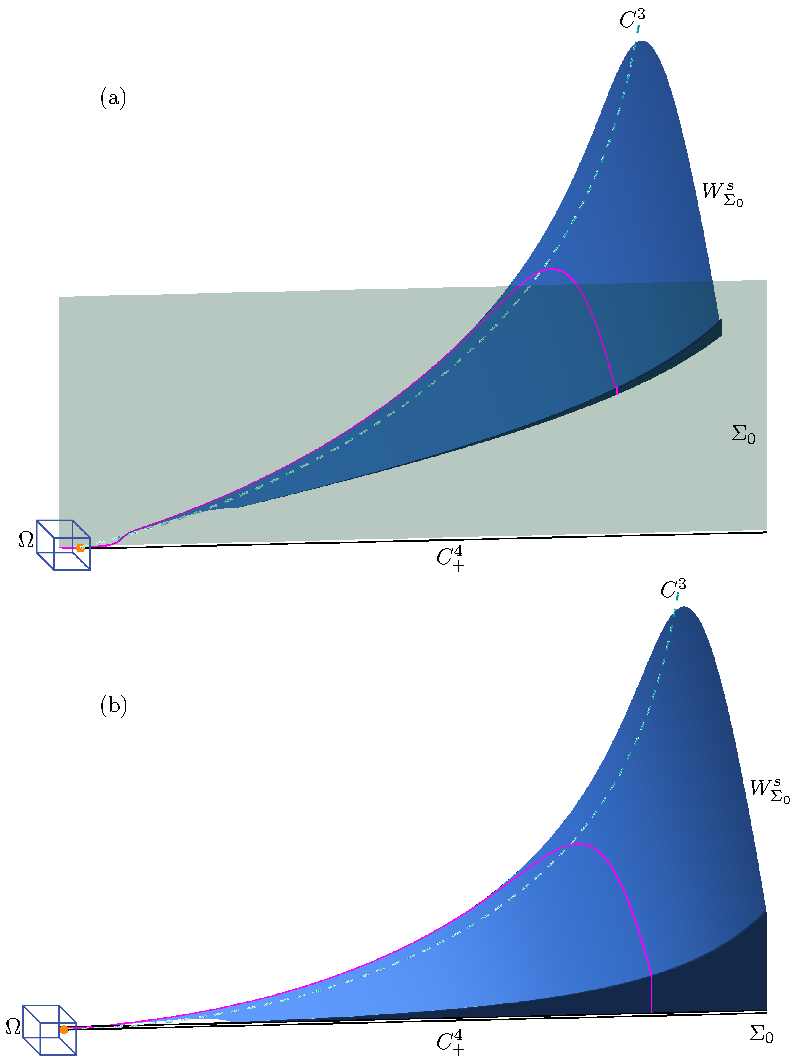
\includegraphics[]{./figures/MKMO_4.pdf}
\caption{The submanifold $W^{s}_{\Sigma_0}$ (light blue surface) of $W^s(S^3)$, shown in projection onto ($B$, $A$, $X$)-space (a) and onto ($B$, $A$, $Y$)-space (b); also shown are a representative orbit segment $\mathbf{u}$ (magenta curve), the plane $\Sigma_0$ (mint surface and line), $\Omega$ (represented by a blue cube), $C^3$, $C^4_+$, and $F_1$.}
\label{figure_4}
\end{figure}



\begin{figure}[H]
\centering
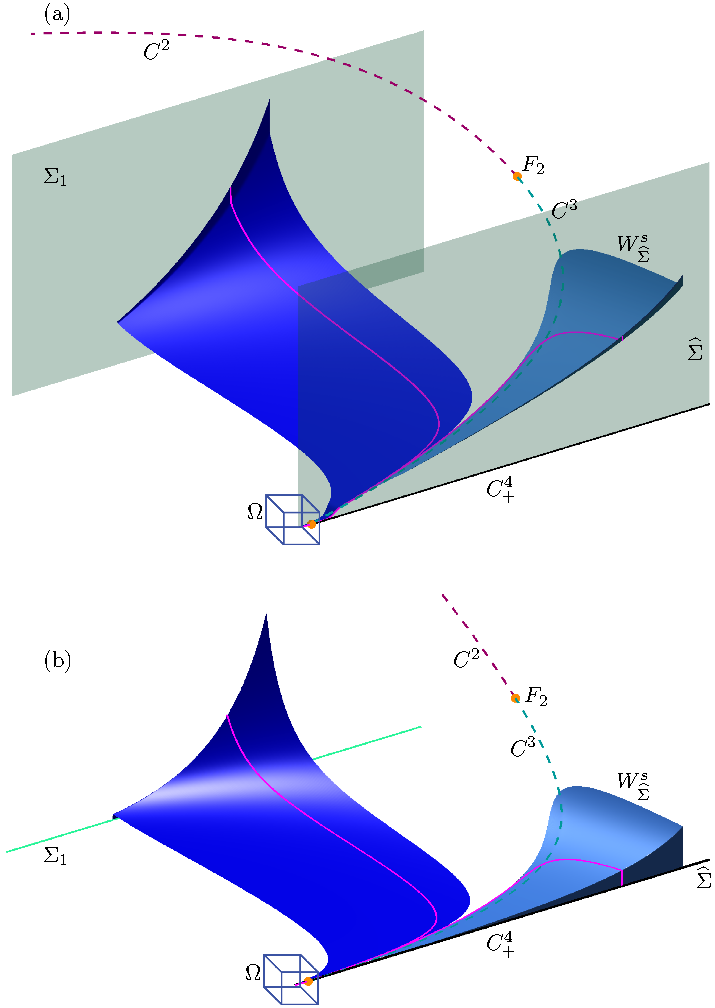
\includegraphics[]{./figures/MKMO_5.pdf}
\caption{The submanifolds $W^{s}_{\Sigma_0}$ (blue surface) and $W^{s}_{\Sigma_0}$ (light blue surface) of $W^s$, shown in projection onto ($B$, $A$, $X$)-space (a) and onto ($B$, $A$, $Y$)-space (b); also shown are representative orbit segments $\mathbf{u}$ (magenta curves), the planes $\Sigma_0$ (mint surface and line) and $\Sigma_1$ (mint surface and line), and $\Omega$ (represented by a blue cube), $C^2$, $C^3$, $C^4_+$, $F_1$, and $F_2$.}
\label{figure_5}
\end{figure}

Figure \ref{figure_5} shows $W^s_{\Sigma_0}$ (light blue surface) together with one other submanifold $W^{s}_{\Sigma_1}$ (blue surface) of $W^{s}$ in projection onto ($B$, $A$, $X$)-space and ($B$, $A$, $Y$)-space; here $\Sigma_1$ (mint surface) is given by $A=2.0$ and $Y=0.0$.  The surface $\Sigma_1$ appears as a line in panel (b) because it is defined by constant $A$ and $X$.  The submanifold $W^s_{\Sigma_1}$ is an example of a submanifold on the other side of $C$ with respect to the variable $A$; compare with Figure 3(d).  A representative magenta orbit segment on $W^s_{\Sigma_1}$ is shown approaching $S^3$ mainly from the $X$- and $Y$-directions, before approaching mostly in the $A$-direction.

\begin{figure}[H]
\centering
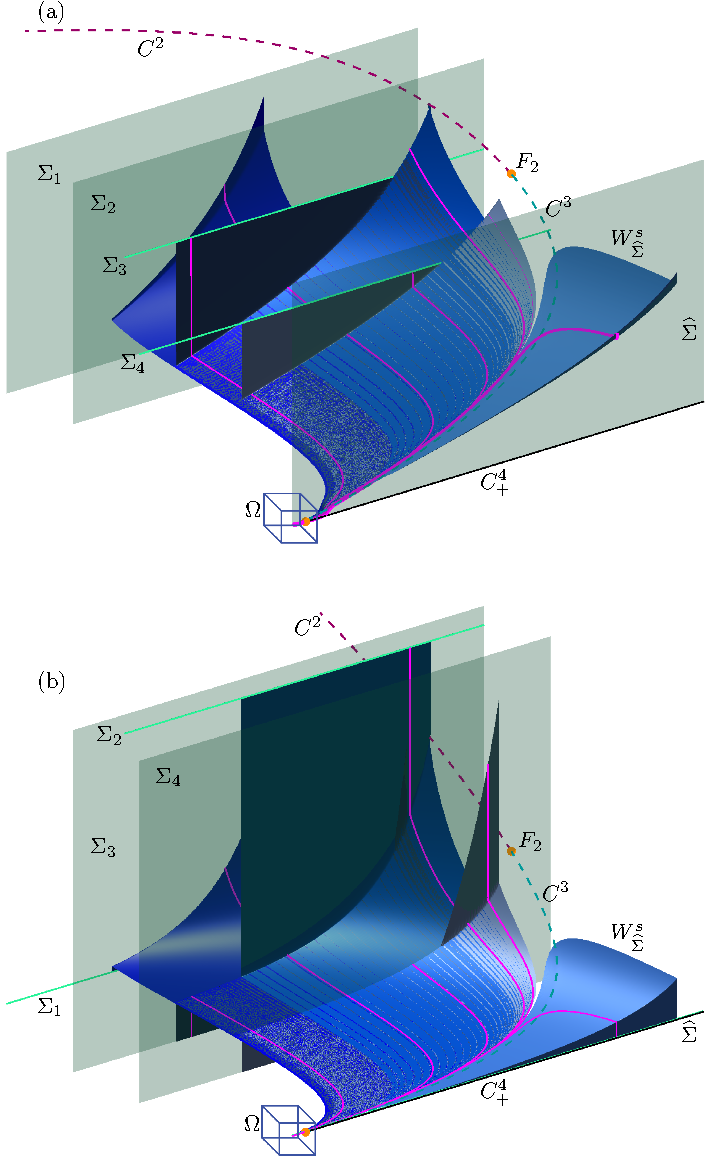
\includegraphics[]{./figures/MKMO_6.pdf}
\caption{The submanifolds from Figure 5 with three additional submanifolds $W^s_{\Sigma_i}$ (blue surfaces) of $W^s$ for $2 \geq i \leq 4$ in projection onto ($B$, $A$, $X$)-space (a) and ($B$, $A$, $Y$)-space (b); also shown are representative orbit segments $\mathbf{u}$ (magenta curves), the planes $\Sigma_i$ (mint surfaces and lines), and $\Omega$ (represented by a blue cube), $C^2$, $C^3$, $C^4_+$, $F_1$, and $F_2$.}
\label{figure_6}
\end{figure}

Figure \ref{figure_6} shows the two submanifolds of $W^{s}$ from Figure \ref{figure_5} with three additional submanifolds $W^s_{\Sigma_i}$ (blue surfaces) and the planes $\Sigma_i$ (mint surfaces) that define them.  Also shown are $C^3$, $C^4_+$, $F_1$, and $\Omega$.  The additional submanifolds were selected with $\Sigma_2$ given by $A=4.0$ and $Y=0.75$, $\Sigma_3$ given by $A=4.0$ and $X=0.75$, and $\Sigma_4$ given by $A=6.0$ and $X=0.5$.  Note that $\Sigma_2$ appears as a line in panel (b) because it is defined by constant values of $A$ and $Y$. Similarly, $\Sigma_3$ and $\Sigma_4$ appear as lines in panel (a) because they are defined by constant $A$ and $X$.  Orbit segments in Figure \ref{figure_6} again approach $S^3$ in the $X$- and $Y$-directions before approaching in the $A$-direction.  This is responsible for regions where different submanifolds are extremely close to each other.  In fact, these surfaces are so close that Matlab cannot distinguish them properly.  Different choices of $B_{\text{in}}$ and $B_{\text{out}}$ also cause some submanifolds to extend farther than others in the $B$-direction.

Overall this section and its figures demonstrate that we can reliably compute any number of submanifolds $W^s_\Sigma$ with conditions (\ref{general_conditions_1}),  (\ref{general_conditions_2}), and (\ref{general_conditions_3}) and the homotopy steps outlined above.  Together, these two-dimensional submanifolds provide an understanding of the dynamics inside $W^s(S^3)$.

%unstable
\subsection{Definition and computation of $W^{u}(S^2)$}  

We can define $S^2$ and $W^u(S^2)$ similarly to how we defined $S^3$ and $W^s(S^3)$.  The values for $B_{\text{in}}$ and $B_{\text{out}}$ are chosen such that $[B_{\text{out}}, B_{\text{in}}] \subset (B_q, B_H)$ where $B_q=0.323$ and $B_H= 0.897$ are the $B$-values of the saddle equilibrium $q$ and the Hopf point $H$ shown, respectively, as a green cross and a pink dot in Figures \ref{figure_1}, \ref{figure_3}, and \ref{figure_7}. Note that in these figures, the flow near $S^2$ is toward $q$; hence, to the right of $W^u(q)$ the flow is to the left.  Our choice of $B_{\text{out}}>B_{q}$ is to avoid a change in direction of the flow associated with $q$.

To compute a submanifold of $W^{u}(S^2)$ we use slightly different boundary conditions and homotopy steps compared to those used for $W^s(S^3)$ in light of two complicating challenges arising from $q$ and $H$.  Orbit segments near $S^2$ may increase in integration time by approaching $W^s(q)$ or by following the attracting slow manifold associated with $C^4_-$ backwards in time.  We define a submanifold of $W^u(S^2)$ with boundary conditions that ensure that computed orbit segments do not demonstrate these behaviours and only increase in integration time by approaching $S^2$.  

To define $S^2$ and $W^s(S^2)$, we define a three-dimensional cylinder $\mathscr{D}^u$ that is transverse to the flow and to $E^s(C^2)$.  To this end, we choose a radius $r$ and for each $B_p \in [B_{\mathrm{in}}, B_{\mathrm{out}}]$ define the two-dimensional sphere in the subspace $\{\omega \in \mathbb{R}^4 \; | \; B=B_p\}$ centred at $p$ and with radius $r$; here $p \in C^2$ is the unique point such that $p_B = B_p$.  More formally,

\begin{equation*}
D^u_r(B_p)=\{w \in \mathbb{R}^4 \;|\; w_B = B_p, \left\lVert w-p \right\lVert  = r\}.
\end{equation*}
Then 
\begin{equation*}
\mathscr{D}^u = \bigcup\limits_{B_p \in [B_{\mathrm{out}}, B_{\mathrm{in}}]}^{}D^u_r(B),
\end{equation*}
is a three-dimensional cylinder.  A smooth, one-parameter family of orbit segments of (\ref{equation_1}) is then given by the property that each orbit segment remains inside $\mathscr{D}^u$ for an O(1) amount of slow time, exits $\mathscr{D}^u$ via $D^u_r(B_p)$ for some $B_p \in [B_{\text{out}}, B_{\text{in}}]$ and ends in some plane $\Sigma$.  We denote by $W^u_\Sigma$ those parts of the orbit segments that exit $\mathscr{D}^u$ in the fast direction.  The earlier parts that evolve mostly in the $B$-direction inside $\mathscr{D}^u$ for $O(1)$ slow time are approximate segments of $S^2$.  If such an earlier part of the orbit segment includes a fast entrance into $\mathscr{D}^u$, that fast part lies on $W^s(S^2)$ in good approximation.

We compute the submanifold $W^u_\Sigma$ again as a one-parameter family of orbit segments $\mathbf{w}$ satisfying the rescaled equation (\ref{equation_4}).  Orbit segments $\mathbf{w} \in W^u_\Sigma$ must satisfy the boundary conditions
\begin{equation}
	\mathbf{w}(1) \in \Sigma,
	\label{general_conditions_unstable_1}
\end{equation}

\begin{equation}
	\mathbf{w}(0) \in \Phi = E^u(p_0) \times \begin{bmatrix} 0, 1, 0, 0 \end{bmatrix}^{tr},
\label{general_conditions_unstable_2}
\end{equation}

\begin{equation}
	\mathbf{w}(0)_B = \widehat{B},
	\label{general_conditions_unstable_3}
\end{equation}
where $p_0 \in C^2$ is such that $p_{0_B} \in (B_{\text{out}}, B_{\text{in}})$ and $\widehat{B}>B_{\text{in}}$.  Equations (\ref{general_conditions_unstable_1}) and (\ref{general_conditions_unstable_2}) are analogous to equations (\ref{general_conditions_1}) and (\ref{general_conditions_2}) from section 3.2.  Equation (\ref{general_conditions_unstable_3}) serves the purpose of preventing $\mathbf{w}$ from increasing in integration time by following the attracting slow manifold associated with $C^4_-$ backwards in time; it has no analogue in section 3.2.    Equations (\ref{general_conditions_unstable_1}), (\ref{general_conditions_unstable_2}), and (\ref{general_conditions_unstable_3}) define four conditions on solutions of (\ref{equation_4}) so that there is a one-parameter family of solutions to this 2PBVP.  We denote the two-dimensional submanifold given by this one-parameter family by $W^u_\Sigma$.

Note that the above conditions preclude the selection of $\mathbf{w}$ with maximal integration time as was done in section 3.2 with equation (\ref{general_conditions_3}).  In the case that we would like to impose a condition of maximum integration time, we may substitute for (\ref{general_conditions_unstable_1}), the two conditions
\begin{equation}
	\mathbf{w}(1) \in \mathscr{D}^u,
	\label{general_conditions_unstable_4}
\end{equation}
and
\begin{equation}
	T = T^B,
	\label{general_conditions_unstable_5}
\end{equation}
where for each $B_p \in [B_{\text{out}}, B_{\text{in}}]$, the time $T^B$ is the maximum integration time of an orbit segment that permanently exits $\mathscr{D}^u$ at $B = B_p$ while satisfying (\ref{general_conditions_unstable_2}) and (\ref{general_conditions_unstable_3}).  Equation (\ref{general_conditions_unstable_4}) imposes one condition on $\mathbf{w}(1)$, one less condition than equation (\ref{general_conditions_unstable_1}), allowing us to also impose equation (\ref{general_conditions_unstable_5}).  Equations (\ref{general_conditions_unstable_2}), (\ref{general_conditions_unstable_3}), (\ref{general_conditions_unstable_4}), and (\ref{general_conditions_unstable_5}) define four conditions on solutions of (\ref{equation_4}) so that there is again a one-parameter family of solutions to this 2PBVP.  We denote the two-dimensional submanifold given by this one-parameter family by $W^u_r$.

Once an initial $\mathbf{w}$ satisfying one of the 2PBVPs  is found, it is possible to sweep out a submanifold $W^u_\Sigma$ or $W^u_r$ by continuing $\mathbf{w}$ with varying $\mathbf{w}(1)_B$ and $T_B$.  The challenge is, once again, the computation via homotopy steps of an initial orbit segment satisfying the boundary conditions.

In the first homotopy step, we choose the point $p_0=\begin{pmatrix} p_{0_A}, p_{0_B}, p_{0_X}, p_{0_Y} \end{pmatrix} \in C^2$ by fixing $p_{0_B}=B_0 \in [B_{\text{out}}, B_{\text{in}}]$.  We impose condition (\ref{general_conditions_unstable_2}) as well as the condition
	\begin{equation}
		\mathbf{w}(1) \in \chi = \{ \omega \in \mathbb{R}^4 \; | \; \omega_A=p_{0_A}, \omega_B=p_{0_B} \omega_Y=p_{0_Y} \}.
		\label{specific_BC_unstable1}
	\end{equation}
The point $p_0$ is then a solution to (\ref{general_conditions_unstable_2}) and (\ref{specific_BC_unstable1}) for $T=0$.  We increase $\mathbf{w}_B$ with $T$ as a free parameter and stop the continuation when $\mathbf{w}_B=\widehat{B}$.  The value of $\mathbf{w}_B$ is fixed from this step onwards.  We define the two-dimensional space

\begin{equation*}
	\Phi_{\widehat{B}} = \Phi \cap \{ \omega \in \mathbb{R} \; | \; \omega_B=\widehat{B}\}.
\end{equation*}

In the second homotopy step, we substitute equation (\ref{specific_BC_unstable1}) for (\ref{general_conditions_unstable_1}) with $\Sigma=\{ \omega \in \mathbb{R}^4 \;|\; \omega_A=p_{0_A}, \omega_Y=p_{0_Y} \}$ and impose (\ref{general_conditions_unstable_3}).  The orbit segment $\mathbf{w}$ at the end of the first homotopy step is then a solution to this 2PBVP defined by (\ref{equation_4}), (\ref{general_conditions_unstable_1}), (\ref{general_conditions_unstable_2}), and (\ref{general_conditions_unstable_3}).  It is in the second homotopy step that we decide whether to compute a submanifold $W^u_\Sigma$ or $W^u_r$.  If our aim is to compute $W^u_\Sigma$, all that remains to compute an initial $\mathbf{w}$ lying on the manifold is to move $\Sigma$ to a desired location as in section 3.2.

To compute $W^u_r$ we increase $T$ until $\mathbf{w}(1) \in \Sigma \cap \mathscr{D}^u$.  This is detected as $\mathbf{w}(1)$ reaching a distance of $r$ away from the point $p \in C^2$ such that $p_B = \mathbf{w}_B$.  We denote the endpoint coordinates $\mathbf{w}(1)_B$ and $\mathbf{w}(1)_X$ by $\widetilde{B}$ and $\widetilde{X}$, respectively, at the end of this step.  

In the event that $D_r(\widetilde{B})$ contains a locus of points at which the flow is tangent to it, we perform a third homotopy step to increase $\widetilde{B}$ until the flow is transverse to $D_r(\widetilde{B})$.  This is achieved by imposing conditions (\ref{general_conditions_unstable_2}), (\ref{general_conditions_unstable_3}), and (\ref{general_conditions_unstable_4}) on $\mathbf{w}$ at the end of the second homotopy step and then increasing $\mathbf{w}_B$ while keeping $T$ as a free parameter.

In the final homotopy step, we replace condition (\ref{general_conditions_unstable_4}) with 
	\begin{equation}
		\mathbf{w}(1) \in \Theta = D^u_r(\widetilde{B}) \cap \{ \omega \in \mathbb{R} \; | \; \omega_X = \widetilde{X} \}.
		\label{specific_BC_unstable2}
	\end{equation}
The orbit segment $\mathbf{w}$ at the end of the second homotopy step (or the third homotopy step if one was necessary) is then a solution to the 2PBVP defined by (\ref{equation_4}), (\ref{general_conditions_unstable_2}), (\ref{general_conditions_unstable_3}), and (\ref{specific_BC_unstable2}).    We then increase $T$ until $T=T^B$, which is detected as a fold in integration time.  The resulting orbit segment $\mathbf{w}$ lies on $W^u_r$.

Once an initial orbit segment $\mathbf{w}$ on either $W^u_\Sigma$ or $W^u_r$ is found, we may sweep out the remaining part of the submanifold by increasing and decreasing $\mathbf{w}_B$ and keeping $T$ as a free parameter.

Figure \ref{figure_7} illustrates in projection onto $(B,A)$-space, the adjusted homotopy steps for computing $W^u_r$.  Each panel shows an enlargement of $C$ from Figure \ref{figure_1} near $C^2$ with additional information for the computation.   We choose $p_0=\begin{pmatrix} 0.940272, && 0.7, && 1.492271, && 1.342954 \end{pmatrix}$ which lies on $C^2$.  In the first homotopy step, we impose condition (\ref{specific_BC_unstable1}), which imposes three conditions on $\mathbf{w}(1)$, as well as condition (\ref{general_conditions_unstable_2}), which imposes one restriction on $\mathbf{w}(0)$.  Panel (a) shows a sketch of an intermediate $\mathbf{w}$ (forest green curve) in the first homotopy step; here the one-dimensional line $\chi$ is sketched in mint and the three-dimensional $\Phi$ is sketched as a mint prism.  The $B$-coordinate of $\mathbf{w}(0)$ is increased with $T$ as a free parameter.  The continuation is stopped when $\mathbf{w}(0)_B=\widehat{B}$ for $\widehat{B}=1.0$.  In the second homotopy step, we impose (\ref{general_conditions_unstable_1}), (\ref{general_conditions_unstable_2}), and (\ref{general_conditions_unstable_3}), increasing $\mathbf{w}(1)_B$ with $T$ as a free parameter until $\mathbf{w}(1)$ intersects $\mathscr{D}^u$ for $r=0.7$.  We are not required to perform an additional homotopy step because $D_r(\widetilde{B})$, in this case, does not contain a locus points at which the flow is tangent to it.  Figure \ref{figure_7}(b) shows a sketch of the numerical set up before the final homotopy step; here the one-dimensional closed curve $\Theta$ is sketched in mint and $\Phi_{\widehat{B}}$ is sketched as a mint cross. We then impose (\ref{general_conditions_unstable_2}), (\ref{general_conditions_unstable_3}), (\ref{general_conditions_unstable_4}) and (\ref{general_conditions_unstable_5}) and increase $T$.  The continuation is stopped when $T=T^B$ which is detected as a fold.  The resulting orbit segment lies on $W^u_r$.  We can then sweep out the rest of the submanifold $W^u_r$ by continuing the fold in integration time for increasing and decreasing $\mathbf{w}(1)_B$.

\begin{figure}[H]
\centering
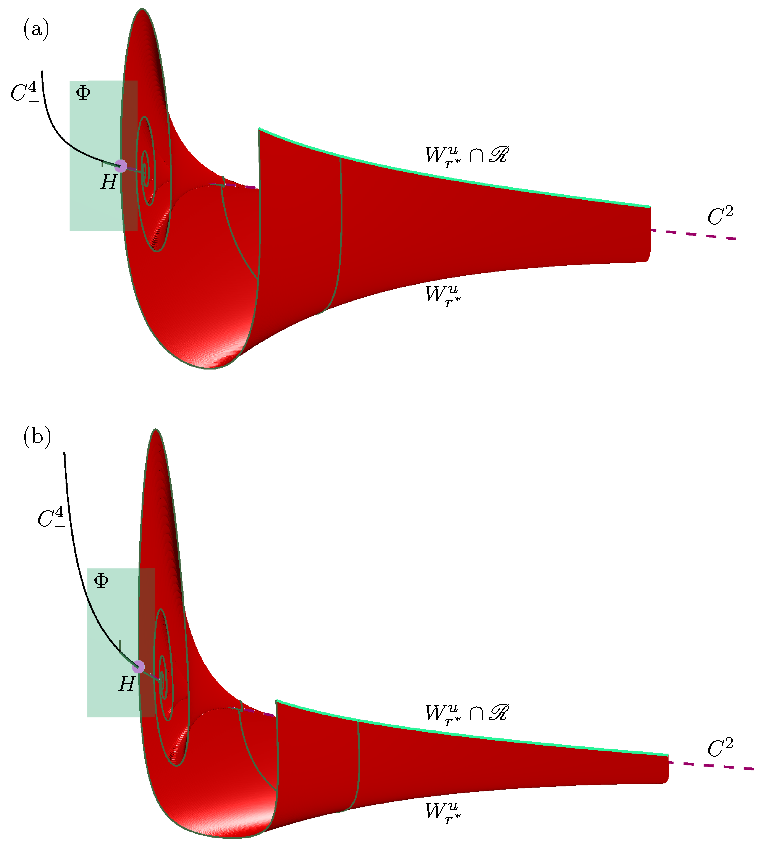
\includegraphics[]{./figures/MKMO_7.pdf}
\caption{A sketch in projection onto the ($B$,$A$)-plane of the homotopy steps for the computation of submanifolds $W^u_r$ of $W^u(S^2)$.  Also shown are $C^2$, $C^4_-$, $H$, $q$, and the orbit segment $\mathbf{w}$ is shown as a forest green curve in each panel.  Panel (a) is a sketch of an intermediate $\mathbf{w}$ in the first homotopy step with $\chi$ (mint line) and $\Phi$ (mint prism); panel (b) is a sketch of the start of the final homotopy step with $\Theta$ (mint circle) and $\Phi_{\widehat{B}}$ (mint cross).}
\label{figure_7}
\end{figure} 

\begin{figure}[H]
\centering
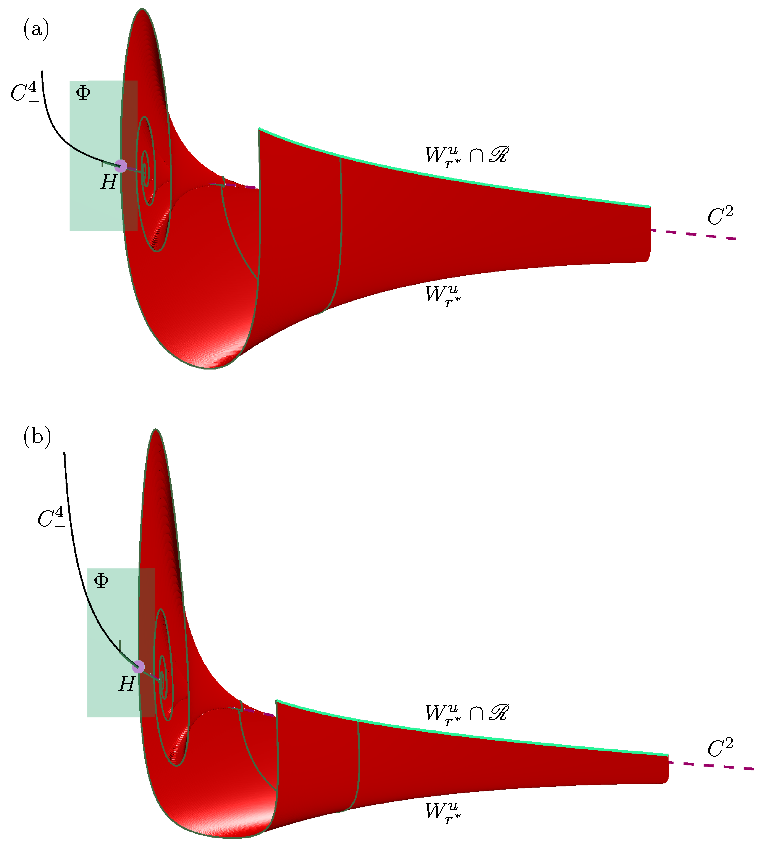
\includegraphics[]{./figures/MKMO_8.pdf}
\caption{The submanifold $W^u_{r}$ (red surface) of $W^u(S^2)$ for $r=0.7$ shown in projection onto $(B,A,X)$-space (a) and $(B,A,Y)$-space (b); note that the view is rotated compared to previous figures.  Also shown are two representative orbit segments $\mathbf{w}$ (forest green curves) on $W^u_{r}$, the two-dimensional space $\Phi_{\widehat{B}}$ (mint surface), the one-dimensional intersection $W^s_{r}\cap\mathscr{D}^u$ (mint curve), and $C^2$, $C^4_-$, and $H$.}
\label{figure_8}
\end{figure}

Figure \ref{figure_8} shows two projections of the submanifold $W^u_{r}$ for $r=0.7$ with $W^u_{r} \cap \mathscr{D}^u$ (mint curve) and $\Phi_{\widehat{B}}$ (mint surface).  Note that $W^u_{r}\cap\mathscr{D}^u$ is simply the curve traced out by $\mathbf{w}(1)$.  To facilitate viewing, the view is rotated compared to previous figures.  Two example orbit segments $\mathbf{w}$ are plotted and a subset of $C^2$ (dashed raspberry curve) is shown.  From this angle, the radius of $\mathscr{D}^u$ may, to some readers, appear to decrease with decreasing $\mathbf{w}(1)_B$.  This is due to the eye's erroneous association of points $\mathbf{w}(1)$ with points $p \in C^2$ such that $p_B < \mathbf{w}(1)_B$.  Due to the spiralling nature of $W^u_r$, we only show one such submanifold for ease of visualization.

%Lin's method

\section{A heteroclinic connection between two saddle slow manifolds}

\begin{figure}[H]
\centering
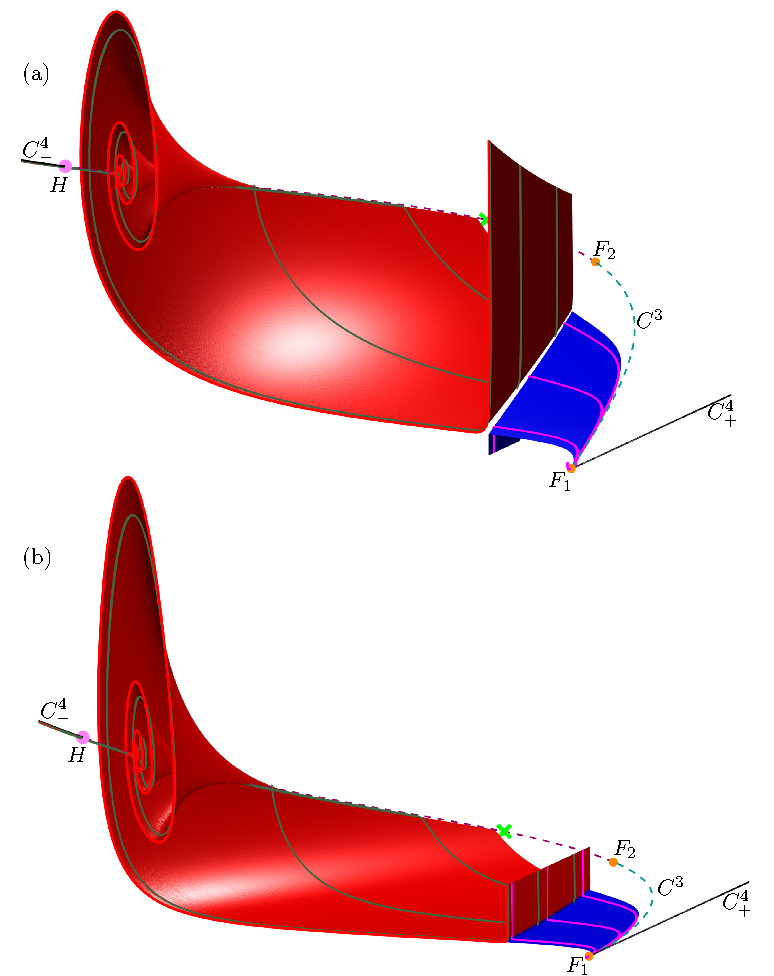
\includegraphics[]{./figures/MKMO_9.pdf}
\caption{The submanifold $W^u_{\Sigma_5}$ (red surface) of $W^u(S^2)$ and the submanifold $W^s_{\Sigma_5}$ (blue surface) of $W^s(S^3)$ in projection onto $(B,A,X)$-space (a) and onto $(B,A,Y)$-space (b). Representative orbit segments $\mathbf{w} \in W^u_{\Sigma_5}$ and $\mathbf{u} \in W^u_{\Sigma_5}$ are plotted in forest green and magenta, respectively; also shown are $C^2$, $C^3$, $C^4_\pm$, $F_1$, $F_2$, $H$, and $q$ (which is partially obscured by the two-dimensional submanifold $W^u_{\Sigma_5}$). }
\label{figure_9}
\end{figure}

The stable manifold of $S^3$ computed for the reduced system in \cite{QSSA} stretches backward in time to reach $S^2$, suggesting the existence of a surface of heteroclinic connections from $S^2$ to $S^3$.  In the full system (\ref{equation_1}), such a surface would be a two-dimensional submanifold of both $W^s(S^3)$ and $W^u(S^2)$ which we denote $\mathscr{H}$.  Supporting the argument for the existence of $\mathscr{H}$ is the fact that two three-dimensional objects in a four-dimensional space  may intersect generically in a two-dimensional manifold.  It follows, then, that the three-dimensional $W^s(S^3)$ and the three-dimensional $W^u(S^2)$ likely intersect in a two-dimensional surface of heteroclinic connections $\mathscr{H}$.  The issue is to see whether this is actually the case by finding the surface of connections $\mathscr{H}$.  A natural way forward is to consider $\mathscr{H}$ as a one-parameter family of concatenations of orbit segments $\mathbf{w} \in W^u(S^2)$ with $\mathbf{u} \in W^u(S^3)$.

A first idea is to compute two two-dimensional submanifolds $W^u_\Sigma$ and $W^s_\Sigma$ up to a suitable choice of a single two-dimensional section $\Sigma$.  However, these two two-dimensional objects do not generically intersect in a four-dimensional space.  Figure \ref{figure_9} demonstrates this difficulty.  The chosen section $\Sigma_5=\{\omega \in \mathbb{R}^4 \;|\; \omega_A= 6.0, \omega_Y=0.5 \}$ yields the submanifolds $W^s_{\Sigma_5}$ (blue surface) and $W^u_{\Sigma_5}$ (red surface) shown in Figure \ref{figure_9}.  Representative orbit segments $\mathbf{w}$ (forest green curves) and $\mathbf{u}$ (magenta curves) are shown coming toward each other mostly in the $A$-direction before diverging away from each other in the faster $X$- and $Y$-directions.  Although the submanifolds appear to intersect in the ($B$, $A$, $Y$)-projection in Figure \ref{figure_9}(b), we can see from the ($B$, $A$, $X$)-projection in Figure \ref{figure_9}(a) that the $W^s_{\Sigma_5}$ and $W^u_{\Sigma_5}$ in fact miss each other in the four-dimensional phase space.  Nevertheless, we are encouraged by the closeness of $W^u_{\Sigma_5}$ and $W^s_{\Sigma_5}$ that suggests that a surface $\mathscr{H}$ of connecting orbits should exist nearby.

We turn to Lin's method to find the actual surface of connecting orbits $\mathscr{H}$.  Lin's method has been used in parameter continuation to locate connections between equilibria and/or periodic orbits \cite{Lin_original, Lin_POs, Lin_POs2}.  We use it here in a novel way to locate structurally stable connections between $S^2$ and $S^3$ for the system parameters given in Table 1.

We begin by choosing a three-dimensional section $\mathscr{L}$, called a Lin section, that divides the four-dimensional phase space into two regions such that $C^3$ lies in one region and $C^2$ lies in the other.  More specifically, the Lin section $\mathscr{L}$ is defined by a constant value of $A$ that is chosen so that $\mathscr{L}$ intersects $C$ to the left of $W^u(q)$ in the ($B$, $A$)-projection; this choice of $\mathscr{L}$ allows us to compute the largest possible portion of $\mathscr{H}$ to the right of $W^u(q)$.  Inside $\mathscr{L}$ we choose a unit vector $\mathbf{v}_Z$ with the generic property that it is not tangent to either $W^u(S^2)$ or $W^s(S^3)$.  The vector $\mathbf{v}_Z$ is called a Lin vector and the space $Z$ spanned by $\mathbf{v}_Z$ the associated Lin space.  We then use the methods outlined in section 3 to compute $\mathbf{u} \in W^s(S^3)$ and $\mathbf{w} \in W^u(S^2)$ such that
\begin{equation}
	\mathbf{u}(0) \in \mathscr{L}
	\label{general_conditions_heteroclinic_1}
\end{equation}
and
\begin{equation}	
	 \mathbf{w}(1) \in \mathscr{L}.
	 \label{general_conditions_heteroclinic_2}
\end{equation}
Additionally, we require that
\begin{equation*}
	\mathbf{u}(0)-\mathbf{w}(1) \in Z.
\end{equation*}
Importantly, the signed distance between $\mathbf{u}(0)$ and $\mathbf{w}(1)$ inside $Z$, given by
\begin{equation}
	\eta=[\mathbf{u}(0)-\mathbf{w}(1)] \cdot \mathbf{v}_Z,
	\label{general_conditions_heteroclinic_3}
\end{equation}
is a regular test function.  Note that $\left\lvert \eta \right\lvert = \left\lVert \mathbf{u}(0)-\mathbf{w}(1) \right\lVert$.  A pair of orbit segments ($\mathbf{w}$, $\mathbf{u}$) with 
\begin{equation}
	\eta = 0
	\label{general_conditions_heteroclinic_4}
\end{equation}
is then a connection between $S^2$ and $S^3$.  Hence, finding a zero of $\eta$ is the way of finding a connecting orbit in $\mathscr{H}$.

To implement $\mathbf{u}(0), \mathbf{w}(1) \in Z$, we define unit normal vectors $\mathbf{n}_1 \perp \mathbf{v}_Z$ and $\mathbf{n}_2 \perp \mathbf{v}_Z$ such that $\mathbf{n}_1 \perp \mathbf{n}_2$ and impose conditions

\begin{equation}
	[\mathbf{u}(0) - \mathbf{w}(1)] \cdot \mathbf{n}_1 =0
	\label{general_conditions_heteroclinic_5}
\end{equation}
and
\begin{equation}	
	 [\mathbf{u}(0) - \mathbf{w}(1)] \cdot \mathbf{n}_2 =0.
	 \label{general_conditions_heteroclinic_6}
\end{equation}
Equations (\ref{general_conditions_heteroclinic_5}) and (\ref{general_conditions_heteroclinic_6}) ensure that $\mathbf{w}(1)-\mathbf{u}(0)$ remains in $Z$.  Conditions (\ref{general_conditions_heteroclinic_3}) and (\ref{general_conditions_heteroclinic_4}) together ensure that $\mathbf{w}(1) = \mathbf{u}(0)$.  Once an initial $(\mathbf{w}, \mathbf{u})$ satisfying the above conditions is found, the surface $\mathscr{H}$ can be swept out, for example by varying $\mathbf{w}(1)_B$ with $\mathbf{u}(0)_B$ and $T$ as additional free parameters.  

The challenge is, as always, the computation via homotopy steps of an initial pair $(\mathbf{w}, \mathbf{u})$ satisfying the required BCs.  In the first homotopy step we compute $\mathbf{w} \in W^u_{\Sigma_{L_1}}$ and $\mathbf{u} \in W^s_{\Sigma_{L_2}}$ for $\Sigma_{L_1} $, $\Sigma_{L_2} \subset \mathscr{L}$, requiring (\ref{general_conditions_1}) and (\ref{specific_BC}) for $\mathbf{u}$ and (\ref{general_conditions_unstable_1}), (\ref{general_conditions_unstable_2}), and (\ref{general_conditions_unstable_3}) for $\mathbf{w}$.  In particular, (\ref{general_conditions_heteroclinic_1}) and (\ref{general_conditions_heteroclinic_2}) are then satisfied and we choose
	\begin{equation*}
		\mathbf{v}_Z = \frac{\mathbf{u}(0) - \mathbf{w}(1)}{\left\lVert \mathbf{u}(0) - \mathbf{w}(1) \right\lVert},
		\label{Lin_vector}
	\end{equation*}
which is a convenient choice of a vector that is (generically) transverse to $W^u(S^2)$ and $W^s(S^3)$. We then find the vectors $\mathbf{n}_1$ and $\mathbf{n}_2$ required for conditions (\ref{general_conditions_heteroclinic_1}) and  (\ref{general_conditions_heteroclinic_2}). Once chosen, the vector $\mathbf{v}_Z$ and normal vectors $\mathbf{n}_1$ and $\mathbf{n}_2$ remains fixed throughout the computations.

The conditions imposed in the first homotopy step define a two-parameter family of orbit segment pairs ($\mathbf{w}$, $\mathbf{u}$) that meet in $\mathscr{L}$ along $Z$.  In the second homotopy step, we now relax conditions (\ref{general_conditions_1}) and (\ref{general_conditions_unstable_1}), which respectively are two conditions each on $\mathbf{u}$ and $\mathbf{w}$, and impose instead conditions (\ref{general_conditions_heteroclinic_1}) and (\ref{general_conditions_heteroclinic_2}), (\ref{general_conditions_heteroclinic_3}), (\ref{general_conditions_heteroclinic_5}) and (\ref{general_conditions_heteroclinic_6}).    Conditions (\ref{general_conditions_heteroclinic_1}) and  (\ref{general_conditions_heteroclinic_2}), respectively, impose one condition on $\mathbf{u}$ and one condition on $\mathbf{w}$.  Conditions  (\ref{general_conditions_heteroclinic_5}) and (\ref{general_conditions_heteroclinic_6}) impose two condition on ($\mathbf{w}$, $\mathbf{u}$).  The number of boundary conditions imposed is hence the same as in the first homotopy step, and thus they define a two-parameter family of orbit segment pairs ($\mathbf{w}$, $\mathbf{u}$).  To choose a one-parameter family ($\mathbf{w}$,$\mathbf{u}$) from these, we impose the additional boundary condition 
	\begin{equation}
		\mathbf{w}(1)_B = B_1,
		\label{specific_BC_hetclin}
	\end{equation}
where $B_1$ is the value of the $B$-coordinate of $\mathbf{w}(1)$ at the end of the first homotopy step.  We now continue $(\mathbf{w}, \mathbf{u})$ as a solution to the 2PBVP defined by (\ref{specific_BC}), (\ref{general_conditions_unstable_2}), (\ref{general_conditions_heteroclinic_1}) and (\ref{general_conditions_heteroclinic_2}), (\ref{general_conditions_heteroclinic_3}) and (\ref{general_conditions_heteroclinic_5}), (\ref{general_conditions_heteroclinic_6}), and (\ref{specific_BC_hetclin}) with $T$ and $\mathbf{u}(0)_B$ as free parameters.  We monitor condition (\ref{general_conditions_heteroclinic_3}) and stop the continuation when $\eta=0$, at which point condition (\ref{general_conditions_heteroclinic_4}) is satisfied and the concatenation of $\mathbf{w}$ with $\mathbf{u}$ is a connecting orbit segment in $\mathscr{H}$.  We can then sweep out the portion of $\mathscr{H}$ to the right of $W^u(q)$ in the ($B$, $A$)-projection by replacing condition (\ref{specific_BC_hetclin}) with (\ref{general_conditions_heteroclinic_4}), keeping $\mathbf{u}(0)_B$, $\mathbf{w}(1)_B$, and $T$ as free parameters.

Figure \ref{figure_10} illustrates, step-by-step in projection onto the ($B$, $A$)-plane, the homotopy steps for computing the portion of $\mathscr{H}$ to the right of $W^u(q)$.  
Each panel shows $C$ from Figure \ref{figure_1} with $\mathscr{L} = \{ \omega \in \mathbb{R}^4 \; | \; \omega_A = 6.0 \}$ (charcoal line), $\mathbf{u} \in W^s_{\Sigma_{L_1}}$ (magenta curve), $\mathbf{w} \in W^u_{\Sigma_{L_2}}$ (forest green curve), the stable eigenspace $E^s(p_{\text{out}})$ (blue cross) from condition (\ref{specific_BC}), the two-dimensional space $\Phi_{\widehat{B}}$ (mint cross) from conditions (\ref{general_conditions_unstable_2}) and (\ref{general_conditions_unstable_3}), and additional information for the computation.  
In the first homotopy step, we choose $\Sigma_{L_1}=\{ \omega \in \mathbb{R}^4 \; | \; \omega_A = 6.0, \omega_Y=-1.0 \}$ and $\Sigma_{L_2}=\{ \omega \in \mathbb{R}^4 \; | \; \omega_A = 6.0, \omega_Y=3.0 \}$.  We compute $\mathbf{w}$ so that $\mathbf{w}(1)_B = B_1 = 0.6$ in the second homotopy step.  Figure \ref{figure_10}(a) is a sketch of the numerical set-up at the end of the first homotopy step.  The points $\mathbf{w}(1)$ and $\mathbf{u}(0)$ lie in the space $Z$ (gold line) from conditions (\ref{general_conditions_heteroclinic_5}) and (\ref{general_conditions_heteroclinic_6}) at a distance $\eta$ from each other.  Panel (b) is a sketch of the numerical set up after the second homotopy step when $\mathbf{w}(1) = \mathbf{u}(0)$ and $\eta=0$.  The resulting pair ($\mathbf{w}$, $\mathbf{u}$) satisfy conditions (\ref{general_conditions_heteroclinic_1}) and (\ref{general_conditions_heteroclinic_2})--(\ref{general_conditions_heteroclinic_4}) and their concatenation lies on the surface $\mathscr{H}$.


\begin{figure}[H]
\centering
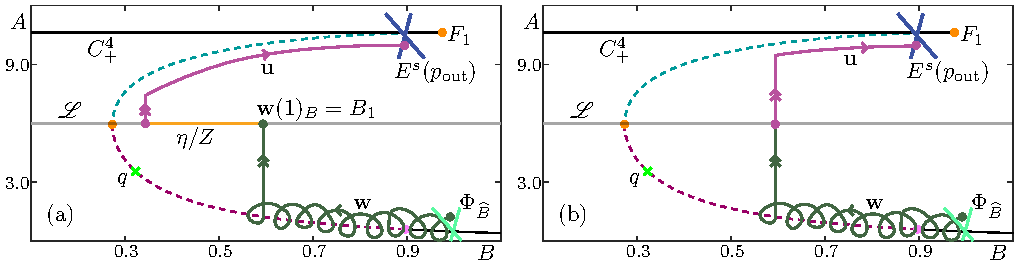
\includegraphics[]{./figures/MKMO_10.pdf}
\caption{A sketch in projection onto the ($B$,$A$)-plane of the numerical set up with Lin's method for the computation of $\mathscr{H}$ to the right of $W^u(q)$.  Also shown are $C^2$, $C^3$, $C^4_\pm$, $F_1$, $F_2$, $H$, and $q$.  Panel (a) shows a sketch at the end of the first homotopy step with $\mathbf{u} \in W^u_{L_1}$ (magenta curve)$, \mathbf{w} \in W^u_{L_2}$ (forest green curve), $\Phi_{\widehat{B}}$ from section 3.2, and the Lin space $Z$ (gold line) in which the points $\mathbf{w}(1)$ and $\mathbf{u}(0)$ lie at a distance $\eta$ from each other.  Panel (b) shows $\mathbf{w}$ and $\mathbf{u}$ after the final homotopy step at which point $\eta=0$ and $\mathbf{w}(1)=\mathbf{u}(0)$.}
\label{figure_10}
\end{figure}

After these homotopy steps we use boundary conditions (\ref{general_conditions_heteroclinic_1}) and (\ref{general_conditions_heteroclinic_2}), (\ref{general_conditions_heteroclinic_3}), (\ref{general_conditions_heteroclinic_4}), and (\ref{general_conditions_heteroclinic_5}) and (\ref{general_conditions_heteroclinic_6}) to sweep out a one-parameter family of orbit segment pairs to obtain an accurate approximation of $\mathscr{H}$ to the right of $W^u(q)$.  Figure \ref{figure_11} shows the computed portion of $\mathscr{H}$ (red/blue surface) with $\mathscr{L}$ (charcoal plane) in projection onto ($B$, $A$, $X$)-space (a) and ($B$, $A$, $Y$)-space (b).  Three concatenated orbit segment pairs ($\mathbf{w}$, $\mathbf{u}$) lying on $\mathscr{H}$ are plotted in forest green for $\mathbf{w}$ and magenta for $\mathbf{u}$.  The portion of the surface swept out by $\mathbf{w}$ is shown in red and that by $\mathbf{u}$ in blue.  Unlike other $W^s_\Sigma$ and $W^u_\Sigma$, ($\mathbf{w}$, $\mathbf{u}$) on $\mathscr{H}$ do not contain segments that diverge quickly in the directions parallel to the $X$- and $Y$-axes.  Orbit segments lying on $\mathscr{H}$ spiral slowly around $S^2$ before crossing the surface at an intermediate speed, mostly in the direction parallel to the $A$-axis to reach and then slowly follow $S^3$.

Figure \ref{figure_12} shows that the computed portion of $\mathscr{H}$ is bounded by $W^u(q)$ (cardinal surface; this surface was computed with the BVP approach outlined in \cite{Red_book}).  Here $\mathscr{H}$ is coloured red near $S^2$ and blue near $S^3$ to illustrate that $\mathscr{H}$ is both a submanifold of $W^u(S^2)$ and of $W^s(S^3)$; compare with Figure \ref{figure_11}.  Similarly, concatenated orbit segments ($\mathbf{w}$, $\mathbf{u}$) are plotted fading from forest green to magenta.  Orbits on $\mathscr{H}$ clearly follow $S^2$ on the slow timescale, before traversing across $\mathscr{H}$ on an intermediate timescale and then following $S^3$ on the slow timescale.  As this figure shows, the saddle point $q$ and its two-dimensional unstable manifold $W^u(q)$ bound the computed portion of $\mathscr{H}$.  Notice how the connecting orbits nearest $W^u(q)$ follow this two-dimensional surface to come very close to $q$, before slowly following $S^2$. Hence, we computed the part of $\mathscr{H}$ to this side of $q$ as closely to $W^u(q)$ as possible.

\begin{figure}[H]
\centering
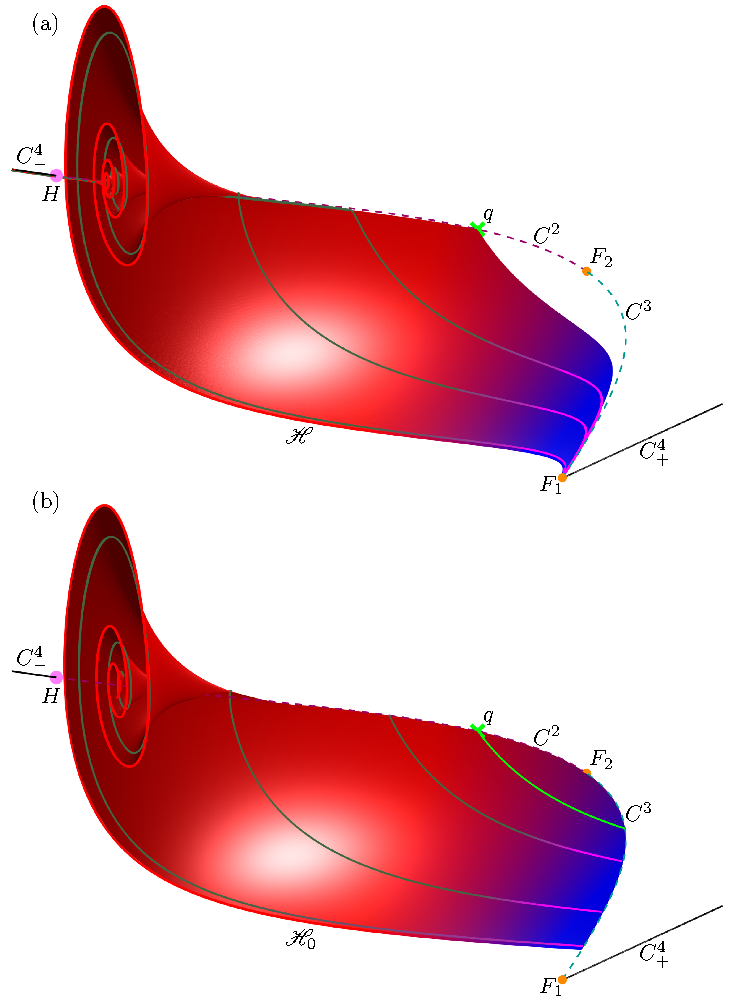
\includegraphics[]{./figures/MKMO_11.pdf}
\caption{The surface of heteroclinic connections $\mathscr{H}$ (red/blue surface) and the Lin section $\mathscr{L}$ (charcoal surface) in projection onto $(B,A,X)$-space (a) and onto $(B,A,Y)$-space (b).  The portion of $W^u(S^2)$ swept out by the $\mathbf{w}$ is shown in red and the portion of $W^s(S^3)$ swept out by the $\mathbf{u}$ is shown in blue.  Also shown are representative orbit segments pairs ($\mathbf{w}$,$\mathbf{u}$) (forest green/magenta curves), $C^2$, $C^3$, $C^4_\pm$, $F_1$, $F_2$, $H$ and $q$ which is partially obscured by $\mathscr{H}$ and $\mathscr{L}$.}
\label{figure_11}
\end{figure}

\begin{figure}[H]
\centering
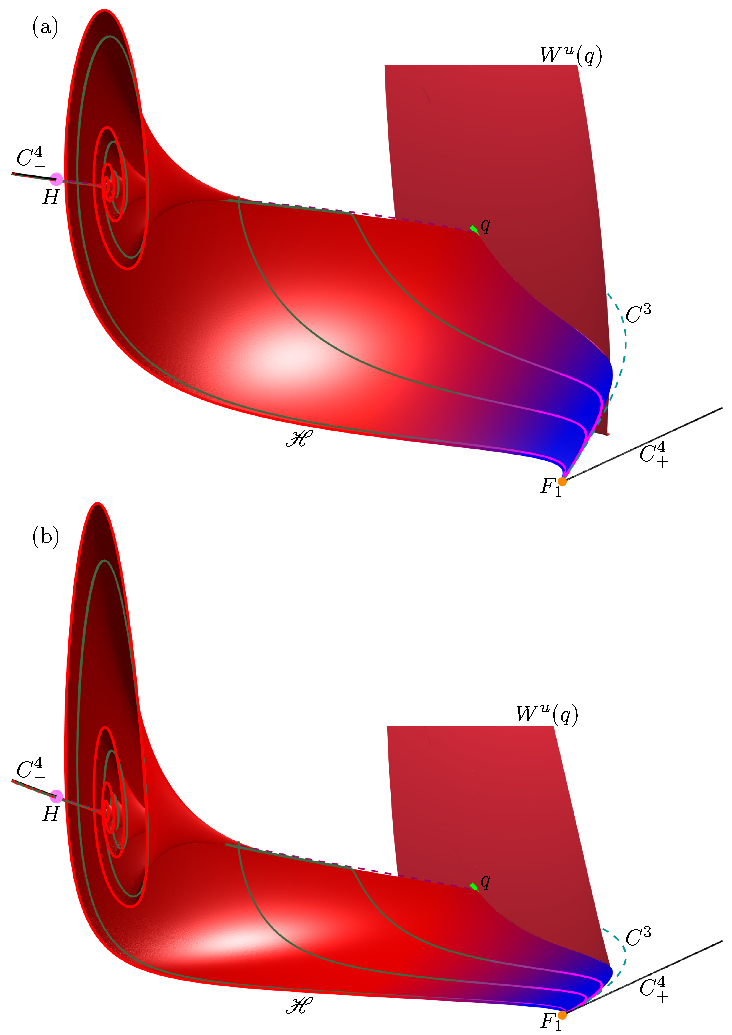
\includegraphics[]{./figures/MKMO_12.pdf}
\caption{The computed portion of $\mathscr{H}$ (red-blue fade surface) is shown in projection onto $(B,A,X)$-space (a) and onto $(B,A,Y)$-space (b) with $W^u(q)$ (cardinal surface).  The unstable manifold $W^u(q)$ bounds the computed portion of $\mathscr{H}$.  Also shown are representative orbit segment pairs ($\mathbf{w}$, $\mathbf{u}$) (forest green-magenta fade curves), $C^2$, $C^3$, $C^4_\pm$, $F_1$, $F_2$, $H$ and $q$ which is partially obscured by $\mathscr{H}$ and $W^u(q)$.  Here $\varepsilon=0.0037$ as in Table 1.}
\label{figure_12}
\end{figure}
%%%%%%%%singular limit surface
\section{Computing the surface of heteroclinic connections in the singular limit}

We now consider the limiting surface $\mathscr{H}_0$ of connecting orbits from $C^2$ to $C^3$ for $\varepsilon = 0$.  Since then system (\ref{equation_1}) reduces to the three-dimensional system (\ref{equation_2}) in which $B$ is a parameter,  the surface $\mathscr{H}_0$ is the one-parameter family, parametrized by $B$, of connections between the saddle equilibria of (\ref{equation_2}) on $C^2$ and on $C^3$, respectively.  It is simple to sweep out $\mathscr{H}_0$ with varying $B$ once an initial connection is found for fixed $B$.  This is exactly the situation addressed in \cite{Red_book} and we now briefly explain how this approach can be used for our purposes.

We compute $\mathscr{H}_0$ as the one parameter family of concatenated of orbit segment pairs, denoted ($\mathbf{w}$, $\mathbf{u}$), of the rescaled system
\begin{equation}
\frac{d\mathbf{u}}{ds} = TG(\mathbf{u}),
\label{fast_rescale}
\end{equation}
where now $\mathbf{u}(s) = (A(s), X(s), Y(s)) \in \mathbb{R}^3$ is the vector of chemical concentrations, $G$ is the right-hand side of (\ref{equation_2}), and $T$ is the integration time on the fast timescale.

We again turn to Lin's method to find an initial orbit segment pair lying on $\mathscr{H}_0$ via homotopy steps.  We begin by choosing a $\widehat{B} \in (B_{\text{in}}, B_{\text{out}})$ corresponding to points $\widehat{p}^2 \in C^2$ and $\widehat{p}^3 \in C^3$.  A two-dimensional Lin section, denoted $\widehat{\mathscr{L}}$, is chosen such that, for any value of $\widehat{B} \in (B_{\text{in}}, B_{\text{out}})$ it divides the three-dimensional phase space into a region containing $\widehat{p}^2$ and a region containing $\widehat{p}^2$.  Inside $\widehat{\mathscr{L}}$, we choose a Lin vector $\mathbf{v}_Z$ with the property that it is not tangent to $W^u(\widehat{p}^2)$ or $W^s(\widehat{p}^3)$.  The Lin vector $\mathbf{v}_Z$ then defines the associated Lin space $Z$.    We then use the methods outlined in \cite{Red_book} to compute $\mathbf{w} \in W^u(\widehat{p}^2)$ and $\mathbf{u} \in W^s(\widehat{p}^3)$ satisfying appropriate boundary conditions.  We first impose two conditions,

\begin{equation}
	\mathbf{u}(1) \in \Upsilon^3= \{ \omega \in \mathbb{R}^3  \; | \; \left\lVert \widehat{p}^3 - \omega \right\lVert = r_3 \} \cap E^s(\widehat{p}^3),
	\label{general_conditions_heteroclinic_singular_1}
\end{equation}
and
\begin{equation}
	\mathbf{w}(0) \in \Upsilon^2= \{ \omega \in \mathbb{R}^3  \; | \; \left\lVert \widehat{p}^2 - \omega \right\lVert = r_2 \} \cap E^u(\widehat{p}^2),
	\label{general_conditions_heteroclinic_singular_2}
\end{equation}

where radii $r_2$ and $r_3$ are chosen such that the closed curves $\Upsilon_2$ and $\Upsilon_3$ are close to $\widehat{p}^2$ and $\widehat{p}^3$, respectively.  We next impose the conditions

\begin{equation}
	\mathbf{u}(0) \in \widehat{\mathscr{L}},
	\label{general_conditions_heteroclinic_singular_3}
\end{equation}
and
\begin{equation}
	\mathbf{w}(1) \in \widehat{\mathscr{L}}
	\label{general_conditions_heteroclinic_singular_4}.
\end{equation}
while additionally requiring that
	\begin{equation*}
		\mathbf{w}(1)-\mathbf{u}(0) \in Z.
	\end{equation*}
The signed distance between $\mathbf{w}(0)$ and $\mathbf{u}(1)$ inside $Z$ is given by
	\begin{equation}
		\eta = [ \mathbf{w}(0)-\mathbf{u}(1) ] \cdot \mathbf{v}_Z
		\label{general_conditions_heteroclinic_singular_5}
	\end{equation}
which is a regular test function.  As before, a pair of orbit segments ($\mathbf{w}$, $\mathbf{u}$) with 
	\begin{equation}
		\eta=0
		\label{general_conditions_heteroclinic_singular_6}
	\end{equation}
is then a connection between $\widehat{p}^2$ and $\widehat{p}^3$.  To implement $\mathbf{u}(0), \mathbf{w}(1) \in Z$, we now define a single unit normal vector $\mathbf{n} \perp \mathbf{v}_Z$ and impose the condition

	\begin{equation}
		[\mathbf{u}(0) - \mathbf{w}(1)] \cdot \mathbf{n} =0
		\label{general_conditions_heteroclinic_singular_7}
	\end{equation}
which ensures that $\mathbf{w}(1)-\mathbf{u}(0)$ remains in $Z$.  Conditions (\ref{general_conditions_heteroclinic_singular_5}) and (\ref{general_conditions_heteroclinic_singular_6}) together ensure that $\mathbf{u}(0)=\mathbf{w}(1)$, while (\ref{general_conditions_heteroclinic_singular_1}) and (\ref{general_conditions_heteroclinic_singular_2}) ensure that $\mathbf{w} \in W^u(\widehat{p}^2)$ and $\mathbf{u} \in W^s(\widehat{p}^3)$.

Again, two homotopy steps are used to find an initial pair ($\mathbf{w}$, $\mathbf{u}$) of connecting orbits.  First, we use the method outlined in \cite{Red_book} to compute $\mathbf{w} \in W^u(\widehat{p}^2)$ and $\mathbf{u} \in W^u(\widehat{p}^3)$ such that (\ref{general_conditions_heteroclinic_singular_3}) and (\ref{general_conditions_heteroclinic_singular_4}) are satisfied; then $\mathbf{w}$ and $\mathbf{u}$ automatically satisfy conditions (\ref{general_conditions_heteroclinic_singular_1}) and (\ref{general_conditions_heteroclinic_singular_2}).  We then choose $\mathbf{v}_Z$ again as

	\begin{equation*}
		\mathbf{v}_Z = \frac{\mathbf{u}(0) - \mathbf{w}(1)}{\left\lVert \mathbf{u}(0) - \mathbf{w}(1) \right\lVert}
		\label{Lin_vector_singular}
	\end{equation*}
and find the unit normal $\mathbf{n}$ required for condition (\ref{general_conditions_heteroclinic_singular_7}); which then remain fixed for throughout the computation.

By construction, the pair ($\mathbf{w}$, $\mathbf{u}$) at the end of the first homotopy step is a solution to the 2PBVP defined by (\ref{general_conditions_heteroclinic_singular_1}), (\ref{general_conditions_heteroclinic_singular_2}), (\ref{general_conditions_heteroclinic_singular_3}), (\ref{general_conditions_heteroclinic_singular_4}), (\ref{general_conditions_heteroclinic_singular_5}), and (\ref{general_conditions_heteroclinic_singular_7}); keeping $\eta$, $T$, $\mathbf{u}(0)_B$, and $\mathbf{w}(1)_B$ as free parameters allows us to close the Lin gap and satisfy $\eta = 0$, at which point the concatenation of $\mathbf{w}$ with $\mathbf{u}$ forms an orbit segment in $\mathscr{H}_0$.

Specifically we choose $\widehat{B}=0.4$, $r_3 = 0.0001$, and $\widehat{\mathscr{L}}=\{ \omega \in \mathbb{R}^4 \; | \omega_A = 6.0\; \}$.  We then sweep out $\mathscr{H}_0$ by imposing condition (\ref{general_conditions_heteroclinic_singular_6}) and increasing and decreasing the parameter $\widehat{B}$, keeping $T$, $\mathbf{w}(1)_B$, $\mathbf{u}(0)_B$, and the coordinates of $\widehat{p}^2$ and $\widehat{p}^3$ as free parameters.  Note that we are not limited by the location of $W^u(q)$ in the computation of $\mathscr{H}_0$.  However, we are faced with an additional challenge due to a change in the type of equilibria on $C^2$ because $q$ is just one of the equilibria on $C^2$.  For $\widehat{B} < 0.476858$, the saddle $\widehat{p}^2$ has real eigenvalues, for $\widehat{B} > 0.476858$ the eigenvalues are complex conjugate, causing spiralling of $\mathbf{w}$ to increase as $\widehat{B}$ approaches $H_B$.  A larger mesh size is needed to numerically approximate $\mathbf{w}$ with more spirals.  On the other hand, keeping the mesh size constant throughout the computation is an advantage when one wants to render the overall surface $\mathscr{H}_0$.  We keep the mesh fixed, but allow the radius $r_2$ to increase as follows
\[r_2= \begin{cases} 
      0.0001 & \widehat {B} < 0.476858 \\
      0.521789(\widehat{B} - 0.476858) + 0.0001 & \widehat {B} < 0.476858
   \end{cases}
\]
Hence, $r_2$ increases linearly from $0.0001$ to $0.2$ between $\widehat{B}=0.476858$ and $\widehat{B}=0.86$, that is, where $p^2$ is complex conjugate. By making $r_2$ larger in this way in regions where orbit segments exhibit more spiralling near $C^2$, we avoid computing tightly spiralling pieces of the orbit segments and thus eliminate the need for a larger mesh size.

\begin{figure}[H]
\centering
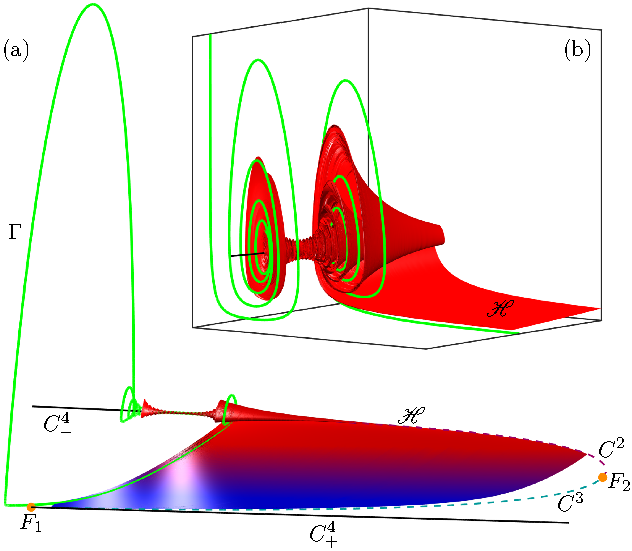
\includegraphics[]{./figures/MKMO_13.pdf}
\caption{Projections onto ($B$, $A$, $X$)-space of the portion of $\mathscr{H}_0$ lying in the region $B < 0.781$ (red-blue fade surface) (a) and of $\mathscr{H}$ for $\varepsilon=0.0037$ (red-blue fade surface) (b).   Also shown in panel (a) for $\varepsilon=0$ are the intersection $W^u(q)\cap\mathscr{H}_0$ (green curve) for $\varepsilon=0$ and the point $p \in C^2$ (periwinkle dot) with $p_B=0.476858$ where the eigenvalues become complex conjugate.    Both panels also show representative orbit segments (forest green-magenta fade curves), $q$, $C^2$, $C^3$, $C^4_\pm$, $F_1$, $F_2$, and $H$.}
\label{figure_13}
\end{figure}

Figure \ref{figure_13} shows in projection into ($B$,$A$,$X$)-space the two computed surfaces $\mathscr{H}_0$ for $\varepsilon=0$ (red-blue fade surface) in panel (a) in comparison with the surface $\mathscr{H}$ for $\varepsilon=0.0037$ (red-blue fade surface) in panel (b) .  To aid a visual comparison with $\mathscr{H}$ in panel (b), we show only the portion of $\mathscr{H}_0$ in panel (a) that lies in the region $B < 0.781$.  Notice how $\mathscr{H}_0$ starts to spiral increasingly from the equilibrium (periwinkle dot) on $C^2$ where the eigenvalues become complex conjugate.  In both panels, three representative orbit segments are shown on the surface (forest green-magenta fade curves).  Unlike orbit segments on $\mathscr{H}$, for $\varepsilon=0$ orbit segments on $\mathscr{H}_0$ do not exhibit any drift in the direction along $C^2$ and $C^3$, respectively.  The intersection of $\mathscr{H}_0$ with $W^u(q)$ (green curve) for $\varepsilon=0$ is analogous to the boundary of $\mathscr{H}$ near $q$; compare with Figure \ref{figure_12}.  Notice that, due to the $B$-dependence of $r_2$, the surface does not spiral all the way into $C^3$ in panel (a).

%%MMO section
\section{Implications for mixed-mode oscillation geometry}

\begin{figure}[H]
\centering
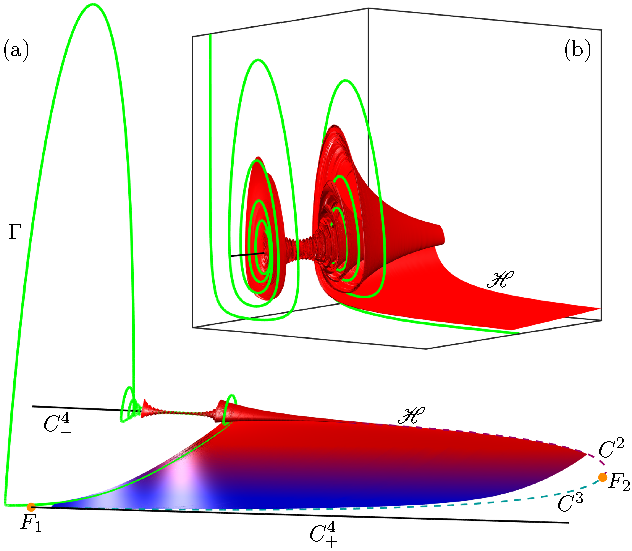
\includegraphics[]{./figures/MKMO_17.pdf}
\caption{The MMO $\Gamma$ (green curve) and the surface of heteroclinic connections $\mathscr{H}$ (red-blue fade surface) shown in projection onto ($B$,$A$,$X$)-space. The surface $\mathscr{H}$ is extended in backwards time past the Hopf bifurcation point $H$.  Panel (a) shows the global view of $\Gamma$ tracking $\mathscr{H}$ from $C^2$ to $C^3$ and making a LAO to $C^4_-$.  Panel (b) shows an enlargement of the region where $\Gamma$ makes a subsequent slow passage through $H$.  Also shown are $q$, $C^2$, $C^3$, $C^4_\pm$, $F_1$, and $F_2$.}
\label{figure_17}
\end{figure}

Figure \ref{figure_17} shows the attracting $\Gamma$ (green curve) for the original value $\varepsilon=0.0037$ in projection into ($B$, $A$, $X$)-space with $\mathscr{H}$ (red-blue fade surface) which is extended in backwards time past $H$.  The MMO $\Gamma$ was obtained by forward time integration.  Figure \ref{figure_17}(a) shows the global view of $\Gamma$.  We observe $\Gamma$ entering into the region of SAOs near the attracting branch $C^4_-$ of $C$.  The MMO spirals as it enters the scroll-like region of $\mathscr{H}$ and makes a slow passage through the Hopf point $H$ to $S^2$.  An enlargement of $\Gamma$'s entry into the scrolls of $\mathscr{H}$ (red surface) and its slow passage through $H$ are shown in inlay (b).  In the enlargement, we also see $\Gamma$ exit the region of SAOs by spiralling out of the scrolls of $\mathscr{H}$ to the underside of the flatter region of $\mathscr{H}$.  In the global view (a), we observe $\Gamma$ subsequently tracking an orbit segment on $\mathscr{H}$ at an intermediate speed in this flatter area of $\mathscr{H}$.  The MMO travels into the blue region of $\mathscr{H}$ before following $S^3$.  Near $F_1$, $\Gamma$ falls off $S^3$ and makes a single LAO back to the attracting slow manifold near $C^4_-$.

\begin{figure}[H]
\centering
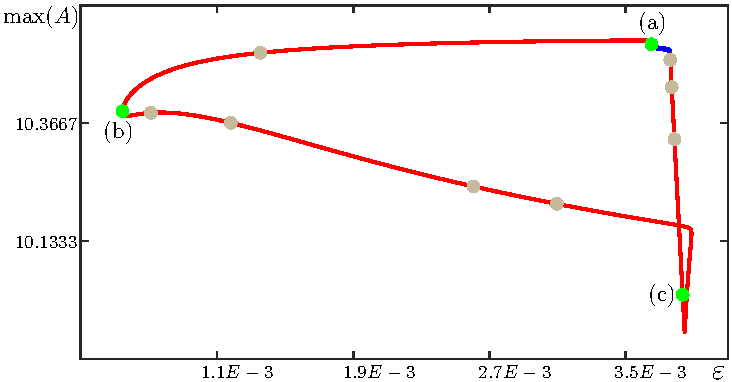
\includegraphics[]{./figures/MKMO_18.pdf}
\caption{The isola of MMO $\Gamma$ over $\varepsilon$.  The PO $\Gamma$ is stable along the blue part and unstable along the red part of the isola.  Green dots labeled (a), (b), and (c) correspond to $\Gamma$ as shown in Figure 14.}
\label{figure_18}
\end{figure}

Having obtained the attracting $\Gamma$ for $\varepsilon=0.0037$, we continue the MMO by varying the time scaling parameter $\varepsilon$.  Figure \ref{figure_18} shows the isola (red and blue curve) of $\Gamma$ over $\varepsilon$, with the vertical axis representing the maximum value of the $A$-coordinate on the MMOs.  The red segment of the isola indicates where $\Gamma$ has at least one unstable Floquet multiplier and the blue segment indicates where $\Gamma$ is stable.  The green dot labeled (a) corresponds to the MMO shown in Figure \ref{figure_17} as well as Figure \ref{figure_18}(a).  Green dots labeled (b), and (c) refer to Figures \ref{figure_15}(b) and  \ref{figure_15}(c), respectively.  Only the green dot labeled (a), corresponding to the original value of epsilon, has an associated $\Gamma$ that is stable.  Mottled pear dots correspond to intermediate $\Gamma$ shown in Figure \ref{figure_20}. The $\Gamma$s associated with the mottled pear dots as well as the $\Gamma$s associated with the green dots labeled (b) and (c) correspond to $\Gamma$ that have at least one unstable Floquet multiplier.


\begin{figure}[H]
\centering
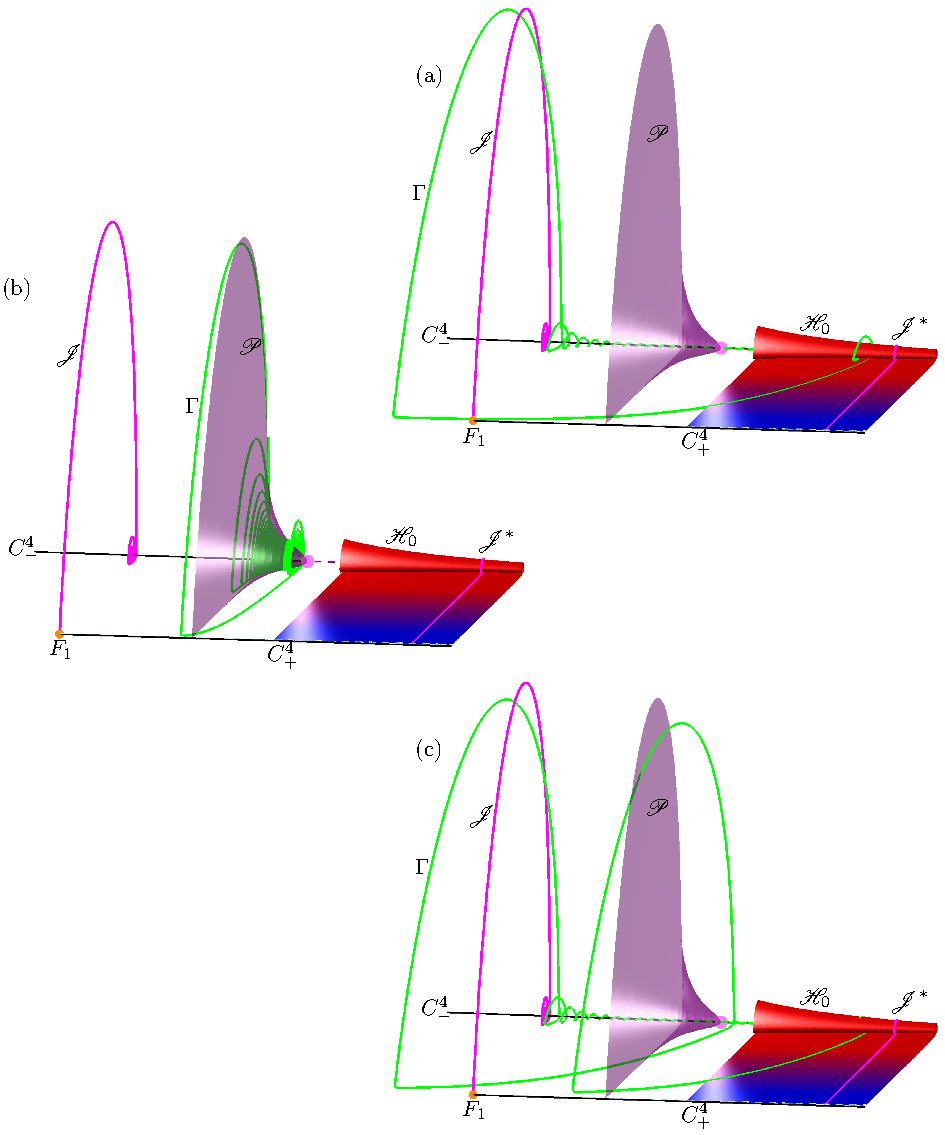
\includegraphics[]{./figures/MKMO_19.pdf}
\caption{Projections onto ($B$, $A$, $X$)-space of the portion of $\mathscr{H}_0$ (red-blue fade surface) lying in the region $B<0.781$, of the jump back trajectory $\mathscr{J}$ (magenta curve) and its dual $\mathscr{J}^*$ (magenta curve), and of the surface of singular POs $\mathscr{P}$ (midnight grape surface).  Also shown are $C^2$, $C^3$, $C^4_\pm$, $F_1$, $F_2$, and $H$.  Panel (a) shows $\Gamma$ (green curve) for the orignal value of $\varepsilon$.  The entry and exit of $\Gamma$ into the region of SAOs are near $\mathscr{J}$ and $\mathscr{J}^*$, respectively.  Panel (b) shows shows a representative $\Gamma$ (green curve) that remains near $\mathscr{P}$ in both the regions of SAOs and LAOs.  Panel (c) shows a representative $\Gamma$ (green curve) that has two LAOs.  Entry and exits into the region of SAOs are again near $\mathscr{J}$ and $\mathscr{J}^*$, respectively.}
\label{figure_19}
\end{figure}

Figure \ref{figure_19} shows $\mathscr{H}_0$ (red-blue fade surface) and several objects of system ($\ref{equation_2}$) with $\Gamma$s (green curves) for different values of $\varepsilon$ in projection into ($B$,$A$,$X$)-space.  A jump back trajectory, denoted by $\mathscr{J}$ (magenta curve), is a heteroclinic connection between equilibria of (\ref{equation_2}) for $B=F_{1_B}$.  It originates at $F_1$ and ends at the attracting equilibrium on $C^4_-$.  The jump back trajectory's dual, $\mathscr{J}^* \in \mathscr{H}_0$ (magenta curve) lies on the other side of and at an equal distance away from $H$.  A one-parameter family in $B$ of singular POs in (\ref{equation_2}) forms a two-dimensional cone, denoted $\mathscr{P}$, is shown in midnight grape.  The cone $\mathscr{P}$ originates from $H$ and terminates in a homoclinic connection of a saddle on $C^3$.  

Panel (a) shows $\Gamma$ for the original value of $\varepsilon=0.0037$, corresponding to the green dot labeled (a) in Figure \ref{figure_18}.  In the ($B$, $A$, $X$)-projection, we see $\Gamma$ making SAOs as it enters the region enclosed by $\mathscr{P}$ and passes the Hopf point $H$ into the scroll-like region of $\mathscr{H}_0$.  The MMO exits the scrolls of $\mathscr{H}_0$ near $\mathscr{J}^*$ to traverse across the flat region of $\mathscr{H}_0$.  Drift in the direction parallel to the $B$-axis causes $\Gamma$ to distance itself from $\mathscr{J}^*$ as it approaches $S^3$.  The MMO then follows $S^3$ until it passes $F_1$, after which it makes an LAO that tracks $\mathscr{J}$ as $\Gamma$ returns to the region of SAOs.

Panel (b) shows $\Gamma$ for $\varepsilon=0.0005$, corresponding to the green dot labeled (b) in Figure \ref{figure_18}.  In the ($B$, $A$, $X$)-projection, we see $\Gamma$ making SAOs in the region enclosed by $\mathscr{P}$.  The SAOs of $\Gamma$ track the singular POs on $\mathscr{P}$ and do not pass through $H$, compare with panel (a).  Instead, $\Gamma$ leaves $C^4_-$ by passing through the surface of $\mathscr{P}$ in the ($B$, $A$, $X$)-projection.  The MMO then travels toward $S^3$ exhibiting minimal drift in the $B$-direction due to the smaller value of $\varepsilon$, compare with panel (a).  Almost immediately after reaching $S^3$, $\Gamma$ makes an LAO that tracks the singular homoclinic connection on $\mathscr{P}$ back to the region of SAOs.

Panel (c) shows $\Gamma$ for $\varepsilon=0.0038$, corresponding to the green dot labeled (c) in Figure \ref{figure_18}. The $\Gamma$ in panel (c) is almost identical to the $\Gamma$ in panel (a) with the exception that it has two LAOs.  The additional LAO back to $C^2$ occurs between $\Gamma$'s exit from region of SAOs along $\mathscr{J}^*$ and the LAO tracking $\mathscr{J}$ back into the region of SAOs.  We regain the drift in the direction parallel to the $B$-axis for the larger value of $\varepsilon$, compare with panel (b).

\begin{figure}[H]
\centering
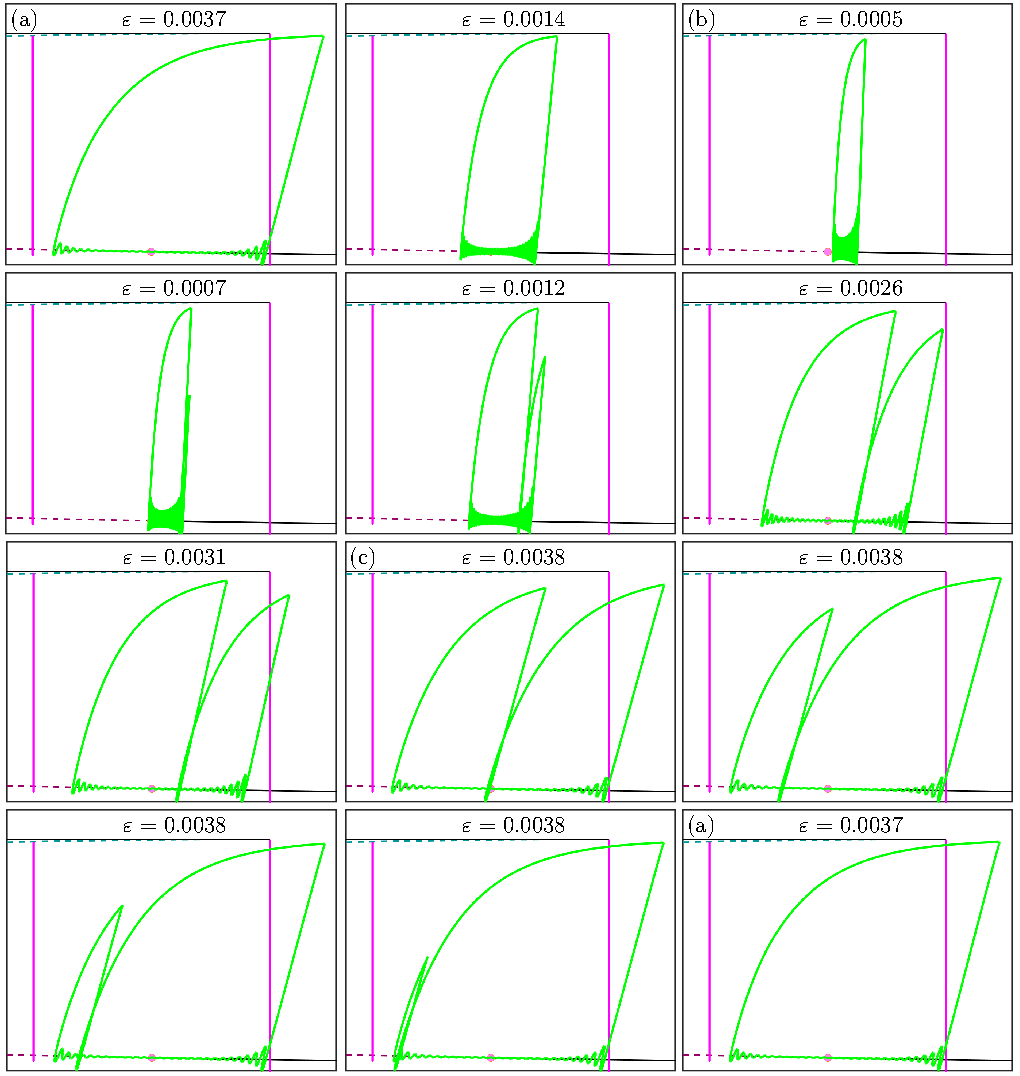
\includegraphics[]{./figures/MKMO_20.pdf}
\caption{Projections onto ($B$, $A$)-plane of $\Gamma$ (green curve) showing the evolution of $\Gamma$ with varying $\varepsilon \in (0.0005, 0.0039)$.  Panels (a), (b), and (c), respectively, correspond to Figures \ref{figure_19}(a), (b), and (c) as well as the green dots with labels (a), (b), and (c) in Figure \ref{figure_18}.  Panels without labels correspond to the taupe dots in Figure \ref{figure_19}.  Also shown are $\mathscr{J}$ and $\mathscr{J}^*$ , $H$, and segments of $C^2$, $C^3$, and $C^4_\pm$.}
\label{figure_20}
\end{figure}

Figure \ref{figure_20} shows $\Gamma$ for several values of $\varepsilon \in (0.0005, 0.0039)$ projected onto the ($A$,$X$)-plane with $\mathscr{J}$ and $\mathscr{J}^*$.  Panels labeled (a), (b), and (c), respectively, correspond to  Figures \ref{figure_19}(a), (b), and (c) as well as green dots labeled (a), (b), and (c) in Figure \ref{figure_18}.  The panels without labels correspond to the unlabeled pear dots in Figure \ref{figure_18}.  They show MMOs for successive values of $\varepsilon$ between those for the MMOs in panels (a), (b), and (c).  The first row of panels in Figure \ref{figure_20} shows the original $\Gamma$ for $\varepsilon=0.0037$ narrowing into the $\Gamma$ for $\varepsilon=0.0005$ in panel (b).  The $\Gamma$ in the intermediate panel corresponds to the pear dot on the upper branch of the isola shown in Figure \ref{figure_18}.  The second row of panels and the first panel in the third row of Figure \ref{figure_20} show an SAO from the $\Gamma$ in panel (b) growing into the second LAO of the $\Gamma$ for $\varepsilon=0.0038$ shown in panel (c).  The $\Gamma$s in the intermediate panels between panel (b) and panel (c) correspond to the pear dots on the lower unstable branch of the isola shown in Figure \ref{figure_18}.  The last two panels of the third row and the first panel of the fourth row show the first LAO from the MMO in panel (c) shrinking into an SAO for the MMO in panel (a).  The $\Gamma$ in the intermediate panels between panel (c) and panel (a) correspond to the pear dots on the nearly vertical branch of the isola shown in Figure \ref{figure_20}.

\section{Conclusions}

We investigated the mechanism for an attracting mixed-mode oscillation (MMO) in the four-dimensional Olsen model for peroxidase-oxidase reaction in a parameter regime corresponding to one slow and two fast variables.  We showed the role of a three-dimensional stable manifold of a saddle slow manifold and a three-dimensional unstable manifold of another saddle slow manifold in the organisation of the MMO's geometry.  We showed how two-dimensional submanifolds of the three-dimensional stable and unstable manifolds can be defined and computed, their geometry revealing a timescale splitting between the fast variables.

We then investigated a surface of heteroclinic connections resulting from the generic intersection of the three-dimensional stable and unstable manifolds.  We showed how to compute such a surface and how the MMO uses the surface to leave a region of small-amplitude oscillations near a delayed Hopf bifurcation in order to reinject itself into a region of large-amplitude oscillations.

We showed how to compute the surface of heteroclinic connections for the singular case in which the time scaling parameter is zero.  The distance between the singular surface and the full system surface was found to be small enough that the singular surface could approximate the full system surface for small values of the time scaling parameter.  We then continued the MMO in the time-scaling parameter to obtain an isola of MMOs and showed how the MMOs on the isola are organised by the singular surface of connections among several other singular objects.

In future we would like to FIGURE OUT FUTURE DIRECTION

\section{Appendix}

\subsection{Distance of $\mathscr{H}$ from $\mathscr{H}_0$}

Fenichel theory states that $\mathscr{H}$ converges to $\mathscr{H}_0$ with decreasing $\varepsilon$ \cite{Fenichel}.  A natural question is then how close $\mathscr{H}_0$ and $\mathscr{H}$ are to each other for $\varepsilon=0.0037$.  To investigate the distance of $\mathscr{H}$ from $\mathscr{H}_0$, we stratify the surfaces into intersections with sections $\Lambda = \{ \omega \in \mathbb{R}^4 \; | \; \omega_B = \widehat{B}\}$ for several values of $\widehat{B}$.  We denote intersections $\mathscr{H} \cap \Lambda := \mathscr{H}^{\widehat{B}}$ and $\mathscr{H}_0 \cap \Lambda := \mathscr{H}_0^{\widehat{B}}$, respectively.  The integral norms between $\mathscr{H}^{\widehat{B}}$ and $\mathscr{H}_0^{\widehat{B}}$ are then computed to give an idea of the distance of $\mathscr{H}$ from $\mathscr{H}_0$.

Any $\mathscr{H}_0^{\widehat{B}}$ can be readily obtained by including the requirement that $B=\widehat{B}$ in the computation of $\mathscr{H}_0$.  Since we do not intend to render a surface after the computation of $\mathscr{H}_0^{\widehat{B}}$, we increase the mesh size in the computation and take $r_2=1\times10^{-3}$.

To compute $\mathscr{H}^{\widehat{B}}$, we could use a computer package such as $\textsc{MATLAB}$ to approximate the intersection curve $\mathscr{H}^{\widehat{B}} = \mathscr{H} \cap \Lambda$ from the data of the computed surface $\mathscr{H}$.  However it is much more accurate and elegant to compute $\mathscr{H}^{\widehat{B}}$ via continuation.  To do so, we follow the steps for computing $\mathscr{H}$ and stop the continuation when $\mathbf{u}(0)_B = \widehat{B}$ instead of sweeping out the entire surface.  We then replace conditions (\ref{general_conditions_heteroclinic_1}) and (\ref{general_conditions_heteroclinic_2}) with the new boundary conditions
	\begin{equation}
		\mathbf{u}(0) \in \Lambda
		\label{general_conditions_intersection_1}
	\end{equation}
and
	\begin{equation}
		\mathbf{w}(0) \in \Lambda
		\label{general_conditions_intersection_2}
	\end{equation}	
and continue the one-parameter family of pairs ($\mathbf{w}$, $\mathbf{u}$) satisfying (\ref{general_conditions_heteroclinic_3}), (\ref{general_conditions_heteroclinic_4}), (\ref{general_conditions_heteroclinic_5}), (\ref{general_conditions_heteroclinic_6}), (\ref{general_conditions_intersection_1}), and (\ref{general_conditions_intersection_2}) with varying $\mathbf{u}(0)_A$ and $T$.  The curve $\mathscr{H}^{\widehat{B}}$ is then given as the one-parameter family $\mathbf{u}(0)$.

\begin{figure}[H]
\centering
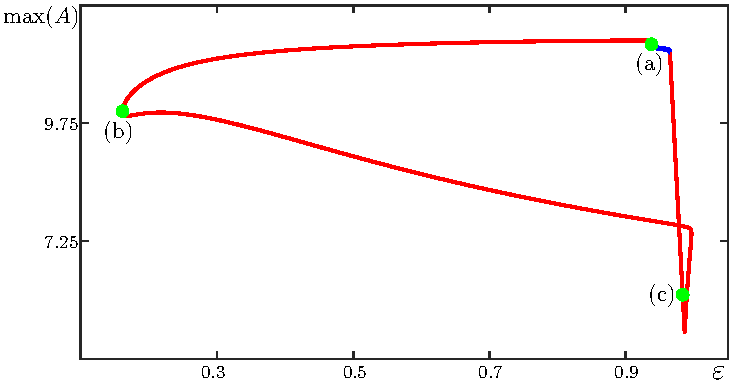
\includegraphics[]{./figures/MKMO_14.pdf}
\caption{Computation of $\mathscr{H}^{\widehat{B}}$ for $\widehat{B}=0.75$ in two parts, shown in projection into ($B$, $A$,$X$)-space.  Panel (a) shows pairs ($\mathbf{w}$,$\mathbf{u}$) where $u$ intersect $\Lambda$ on the righthand side.  Panel (b) shows pairs ($\mathbf{w}$,$\mathbf{u}$) where $u$ intersect $\Lambda$ on the lefthand side.  The pieces were computed as a one-parameter family of ($\mathbf{w}$, $\mathbf{u}$) (forest green/magenta curves) with $\mathbf{u}(0)$ capturing the first intersection of ($\mathbf{w}$, $\mathbf{u}$) with $\Lambda$ (charcoal surface) (a) and with $\mathbf{u}(0)$ capturing the second intersection of ($\mathbf{w}$, $\mathbf{u}$) with $\Lambda$ (b).  Global views of the pieces of $\mathscr{H}$ are shown in panels (a1) and (b1).  Enlargements of the region near $\mathscr{H} \cap \Lambda$ are shown in panels (a2) and (b2).  The full surface $\mathscr{H}$ is not computed in either panel due to the backwards time contraction near $C^2$ rendering the $\mathbf{u}(0)$ near $C^2$ indistinguishable for different ($\mathbf{w}$, $\mathbf{u}$) pairs.  Also shown are two representative ($\mathbf{w}$, $\mathbf{u}$) pairs (forest green/magenta curves), $q$, $C^2$, $C^3$, $C^4_\pm$, $F_1$, $F_2$, and $H$.}
\label{figure_14}
\end{figure}

The three-dimensional section $\Lambda$ is divided into two regions by a two-dimensional surface of points at which the vector field (\ref{equation_1}) is tangent to $\Lambda$ in the $B$-direction.  This surface, called a tangency locus \cite{tangency_locus_paper}, slices the curve $\mathscr{H}^{\widehat{B}}$ into two parts: one on which the vector field (\ref{equation_1}) flows from left to right (from larger to smaller values of $B$) through $\mathscr{H}^{\widehat{B}}$ and the other on which the vector field flows from right to left.  The two pieces of $\mathscr{H}^{\widehat{B}}$ correspond to two pieces of $\mathscr{H}$ which are distinguished by the properties of the pairs ($\mathbf{w}$, $\mathbf{u}$).  Each panel of Figure \ref{figure_14} shows one of the two pieces of $\mathscr{H}$ computed for $\widehat{B}=0.75$ with $\mathbf{w}$ plotted in red and $\mathbf{u}$ plotted in blue.  Panel (a1) shows a global view of the portion of $\mathscr{H}$ for which the flow moves from left to right through $\mathbf{u}(0) \in \mathscr{H}^{\widehat{B}}$.  Panel (a2) shows an enlargement of the region where $\mathscr{H}$ intersects $\Lambda$.  An example orbit segment is shown in forest green and magenta and we can see that $\mathbf{u}(0)$ is on the spiralling region of $\mathscr{H}$. Panel (b1) shows a global view of the portion of $\mathscr{H}$ for which the flow through $\mathbf{u}(0)$ moves from right to left.  Panel (b2) shows an enlargement of the region where $\mathscr{H}$ intersects $\Lambda$ and we can see from an example orbit segment that $\mathbf{u}(0)$ is in a non-spiralling region of $\mathscr{H}$.  The pieces of $\mathscr{H}$ shown in Figure \ref{figure_14}(a1) and Figure \ref{figure_14}(b1) do not constitute the entire surface $\mathscr{H}$.  This is due to the strong contraction in backwards time near $C^2$ that causes many ($\mathbf{w}$, $\mathbf{u}$) pairs to have $\mathbf{u}(0)$ that are not numerically distinguishable.  The pieces of the blue orbit segments $\mathbf{u}$ that are to the right of $\Lambda$ in panels (a1) and (a2) correspond to the red orbit segments to the right of $\Lambda$ in panels (b1) and (b2).  Our algorithm is able to compute both pieces of $\mathscr{H}^{\widehat{B}}$ corresponding to the pieces of $\mathscr{H}$ shown in Figure \ref{figure_14} in one run.

\begin{figure}[H]
\centering
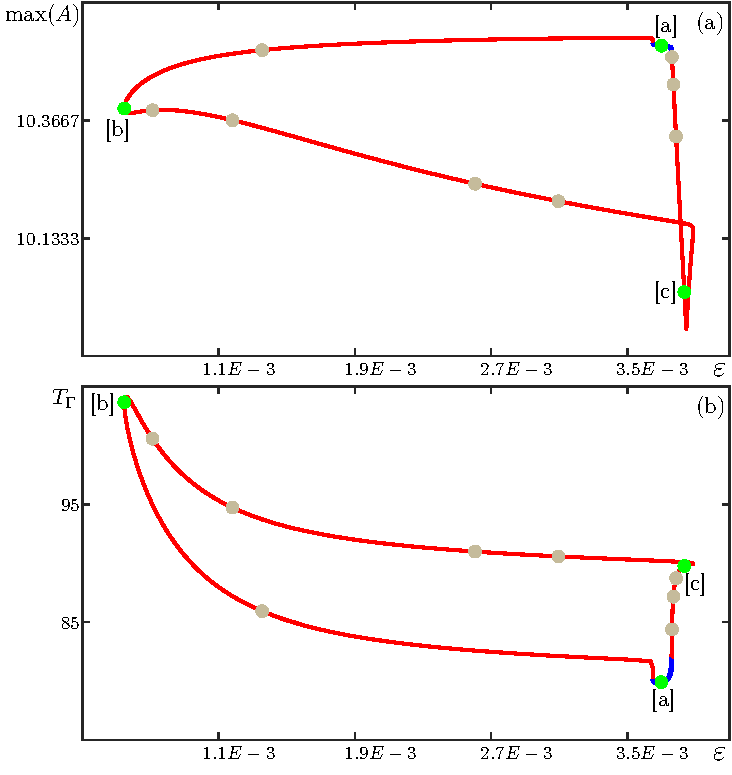
\includegraphics[]{./figures/MKMO_15.pdf}
\caption{Projection into the ($A$, $X$)-plane of the intersection curves $\mathscr{H}^{\widehat{B}}$ (royal purple) and $\mathscr{H}_0^{\widehat{B}}$ (green) of $\mathscr{H}$ and $\mathscr{H}_0$ the with section $\Lambda$ for $\widehat{B}=0.8$, $\widehat{B}=0.75$, $\widehat{B}=0.62$, and $\widehat{B}=0.4$ (front to back).  The curve $\mathscr{H}^{\widehat{B}}$ is visible behind $\mathscr{H}^{\widehat{B}}$ only in the region where the curves are spiralling.}
\label{figure_15}
\end{figure}

Figure \ref{figure_15} shows several curves $\mathscr{H}_0^{\widehat{B}}$ (green) and $\mathscr{H}^{\widehat{B}}$ (purple) given by $\widehat{B}=0.8$, $\widehat{B}=0.75$, $\widehat{B}=0.62$, and $\widehat{B}=0.4$ (front to back) in projection into ($B$, $A$, $X$)-space.  In areas where \textsc{Matlab} cannot distinguish $\mathscr{H}_0^{\widehat{B}}$ from $\mathscr{H}^{\widehat{B}}$, the curves are green.  We can see that curves differ the most in regions where they are spiralling and that more spirals correspond to a larger distance between the curves.  The difference in $\mathscr{H}^{\widehat{B}}$ and $\mathscr{H}_0^{\widehat{B}}$ is more pronounced for $\widehat{B}$ closer to $H_B$ because $\mathscr{H}^{\widehat{B}}$ and $\mathscr{H}_0^{\widehat{B}}$ spiral more as $\widehat{B}$ approaches $H_B$.  In the case of $\widehat{B}=0.4$, it can also be seen that the boundary points of $\mathscr{H}^{\widehat{B}}$ are not the same as and in fact extend past, $\mathscr{H}_0^{\widehat{B}}$.  This is due to $S^3$ and $S^2$ being $O(\varepsilon)$ away from $C^3$ and $C^2$, respectively.

To compare $\mathscr{H}^{\widehat{B}}$ and $\mathscr{H}_0^{\widehat{B}}$ we assign a mesh to $\mathscr{H}_0^{\widehat{B}}$ and index mesh points $l_i$ starting from the boundary point of $\mathscr{H}_0^{\widehat{B}}$ closest to $C^3$.  For each of the $N$ mesh points $l_i \in \mathscr{H}_0^{\widehat{B}}$ we find an associated point $k_i \in \mathscr{H}^{\widehat{B}}$. Assigning a mesh to $\mathscr{H}_0^{\widehat{B}}$ instead of $\mathscr{H}^{\widehat{B}}$ allows us to compare $\mathscr{H}_0$ and $\mathscr{H}$  for different values of $\varepsilon$.  The norm is then the average distance between the point pairs.  This is the discretisation of the integral norm that can be written as the sum
	\begin{equation}
		d := \frac{1}{N} \sum_{i=1}^{N} \left \lVert l_i - k_i\right \lVert,
		\label{integral_norm}
	\end{equation}

To make an appropriate choice of $k_i$ for each $l_i$ in a mesh on $\mathscr{H}^{\widehat{B}}$, we first define the plane $\mathscr{N}_i$ that is normal to $\mathscr{H}_0^{\widehat{B}}$ at the point $l_i$.  The point $k_i$ is then taken to be the intersection $\mathscr{N}_i \cap \mathscr{H}^{\widehat{B}}$.

The points on the pieces of $\mathscr{H}_0^{\widehat{B}}$ that extend past $\mathscr{H}^{\widehat{B}}$ will not have matches on the curve $\mathscr{H}_0^{\widehat{B}}$.  In the flat region, we truncate $\mathscr{H}_0^{\widehat{B}}$ at the first data point such that the plane normal to the data point intersects $\mathscr{H}^{\widehat{B}}$.  We denote the distance between the boundary points of $\mathscr{H}_0^{\widehat{B}}$ and $\mathscr{H}^{\widehat{B}}$ in the spiralling region by $\Delta$.  We then truncate $\mathscr{H}_0^{\widehat{B}}$ at the last data point that has distance greater than $2\Delta$ from the boundary point of $\mathscr{H}^{\widehat{B}}$ in the spiralling region.

\begin{figure}[H]
\centering
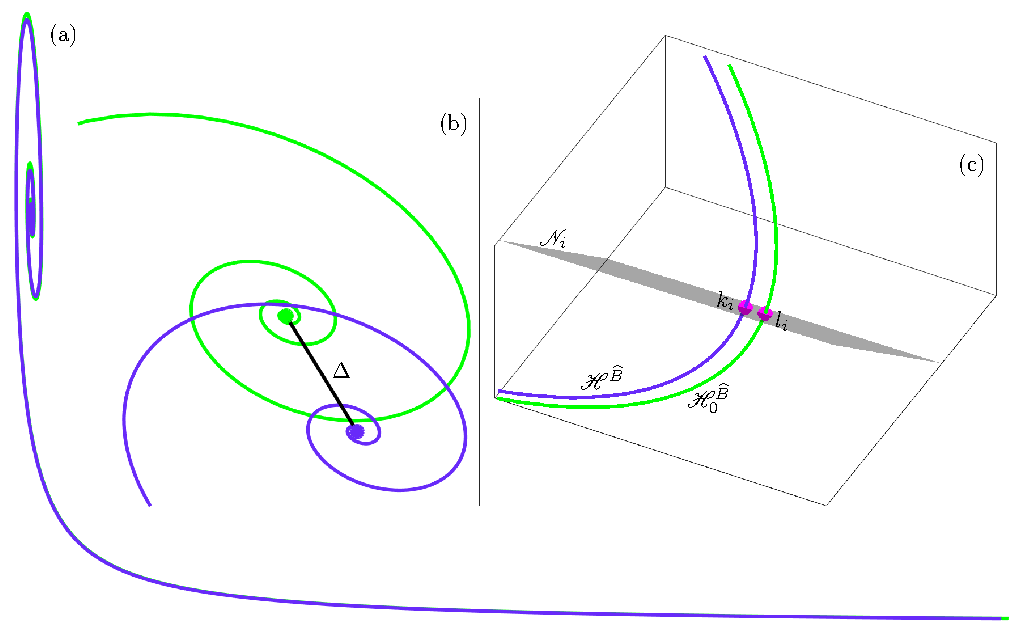
\includegraphics[]{./figures/MKMO_16.pdf}
\caption{Intersection curves $\mathscr{H}^{\widehat{B}}$ (royal purple) and $\mathscr{H}_0^{\widehat{B}}$ (green) for $\widehat{B}=0.75$ projected onto the ($A$, $X$)-plane (a).  An enlargement of the spiralling region near the endpoints of the curves is shown in panel (b) with the line of length $d$ connecting them.  Panel (c) shows a further enlargement of the spiralling region inside the ($A$, $X$, $Y$)-space, $\Lambda$, with the plane $\mathscr{N}_i$ (charcoal surface) that is normal to $\mathscr{H}_0^{\widehat{B}}$ at the point $l_i$ (magenta dot).  The corresponding point $k_i$ on $\mathscr{H}^{\widehat{B}}$ is also shown in magenta.}
\label{figure_16}
\end{figure}

Figure \ref{figure_16}(a) shows $\mathscr{H}_0^{\widehat{B}}$ for $\widehat{B}=0.75$ (green curve) projected onto the ($A$, $X$)-plane, although it is mostly obstructed by $\mathscr{H}^{\widehat{B}}$ (purple curve).  The right-hand endpoint of $\mathscr{H}_0^{\widehat{B}}$ extends past $\mathscr{H}^{\widehat{B}}$ in the ($A$, $X$)-projection.  We truncate in the flat region $\mathscr{H}_0^{\widehat{B}}$ as described above.  Panel (b) shows an enlargement of the spiralling region.  The distance, $\Delta=0.009796$, between the boundary points of $\mathscr{H}_0^{\widehat{B}}$ (green dot) and $\mathscr{H}^{\widehat{B}}$ (purple dot) is represented by a connecting black line.  We truncate the curve $\mathscr{H}_0^{\widehat{B}}$ in the spiralling region as above.  With the built in \textsc{Matlab} function \textsc{spline}, we fit splines $Spl_0$ and $Spl$ to the truncated $\mathscr{H}_0^{\widehat{B}}$ and to $\mathscr{H}^{\widehat{B}}$, respectively.  We then choose a mesh on $\mathscr{H}_0^{\widehat{B}}$ to be the set of computed data points.  For each data point $l_i$, we compute $\mathscr{N}_i$ by applying the built-in \textsc{Matlab} function \textsc{fnder} to $Spl_0$ to obtain a unit tangent vector.  The tangent vector is then used to define two normal vectors spanning $\mathscr{N}_i$.  Points $k_i$ are chosen to be the intersection of the function $Spl$ with $\mathscr{N}_i$. Panel (c) shows a further enlargement of $\mathscr{H}_0^{\widehat{B}}$ and $\mathscr{H}^{\widehat{B}}$ where an example ($l_i$, $k_i$) pair (magenta dots) are shown with the corresponding $\mathscr{N}_i$ (charcoal plane).

We encounter the challenge that some $\mathscr{N}_i$ do not intersect $\mathscr{H}^{\widehat{B}}$.  For these $i$, we omit the point $l_i$ from our computation and lower the mesh size $N$ by one.  Another challenge is that some $\mathscr{N}_i$ have several intersections with $\mathscr{H}^{\widehat{B}}$.  For these values of $i$ we choose $k_i$ to be the intersection with the smallest arclength distance from $k_{i-1}$.  The surface $\mathscr{N}_1$ has only one intersection with $\mathscr{H}^{\widehat{B}}$, so our choice is well defined.  A third issue is that some points $k_i$ are outside the convolute of $Spl_0$, however we include these points in our computation.  Figure \ref{figure_16}(c) shows an enlargement of $\mathscr{H}_0^{\widehat{B}}$ and $\mathscr{H}^{\widehat{B}}$ where an example ($l_i$, $k_i$) pair are shown as magenta dots lying on $\mathscr{H}_0^{\widehat{B}}$ and $\mathscr{H}^{\widehat{B}}$, respectively.  With this method, the approximated integral norm between the $\mathscr{H}_0^{\widehat{B}}$ and $\mathscr{H}^{\widehat{B}}$ for $\widehat{B} = 0.75$ is $7.63856 \times 10^{-3}$.



























  The integral norm is $findthislater$ for $\widehat{B} = 0.8$, $1.153728 \times 10^{-2}$ for $\widehat{B} = 0.62$, and $4.62565 \times 10^{-4}$ for $\widehat{B} = 0.4$.  Note that in this view $\mathscr{H}^{\widehat{B}}$ and $\mathscr{H}_0^{\widehat{B}}$ given by $\widehat{B}=0.75$ are slightly obscured by the curves given by $\widehat{B}=0.8$.

Having sampled the distances between $\mathscr{H}_0^{\widehat{B}}$ and $\mathscr{H}^{\widehat{B}}$ for four $\Lambda$, it is reasonable to assume that $\mathscr{H}$ and $\mathscr{H}_0$ are near enough to each other that $\mathscr{H}_0$ may be used to approximate $\mathscr{H}$ for $\varepsilon << 1$.  This is particularly useful in the next section where we investigate the role of $\mathscr{H}$ in the organization of the MMO $\Gamma$.




\newpage
\bibliography{elle}

\end{document}